% zweiseitiger druck -> bindung
\documentclass[a4paper,10pt,twoside,ngerman,bibliography=totoc]{scrreprt}
% einseitiger druck -> ebook
% \documentclass[a4paper,11pt,oneside,ngerman,bibliography=totoc]{scrreprt}

\usepackage[english]{babel}                          % deutsche Trennmuster
% \usepackage{ae}                           % beseitigt Fehler beim pdf erzeugen

\usepackage[T1]{fontenc}                    % T1-kodierte Schriften, korrekte Trennmuster fuer Worte mit Umlauten
\usepackage[utf8]{inputenc}
\usepackage[default]{opensans}
\usepackage{courier}                        % Courier\ttdefault
\usepackage{microtype}
\usepackage{mathswap}

\usepackage{amsmath,amsthm,amsfonts,amssymb}
\usepackage{esint}                          %schöne integrale, benötigt amsmath

\usepackage{wrapfig}                        % text um bilder fliesen lassen
\usepackage{longtable}
\usepackage{booktabs}
\usepackage{color}                          % Schriftfarbe
\usepackage{lscape}
\usepackage{subcaption}
\usepackage[subfigure]{tocloft}
\usepackage{appendix}
\usepackage{caption}
\usepackage{graphicx}
\usepackage{setspace}
\usepackage{pdfpages}
\usepackage{verbatim}
\usepackage[tight,ugly]{units}
% \usepackage{lmodern}
\usepackage[hidelinks]{hyperref}              %links an referenzen setzen
\usepackage{pgfplots}
\pgfplotsset{compat=1.15}

\usepackage{siunitx}
\usepackage{float}
\usepackage{placeins}
% packages für Programmablaufplan
\usepackage{tikz}
\usetikzlibrary{shapes,arrows}
\usepgflibrary{arrows}


\usepackage{pgf-umlsd}
\usepackage{algorithm}
\usepackage{algorithmic}
\DeclareMathOperator*{\argmax}{arg\,max}


%plus(minus)
% \usepackage{relsize}
% \newcommand*\myPM{\ensuremath{\substack{+\\[-0.25em]-}\,}}
% \newcommand*\myPMbM{\ensuremath{\substack{+\\[-0.25em]\mathsmaller(-\mathsmaller)}\,}}
% \newcommand*\myPMbP{\ensuremath{\substack{\mathsmaller(+\mathsmaller)\\[-0.25em]-}\,}}

% defninierte Farben
\definecolor{fond}{RGB}{240,240,240}

\renewcommand{\vec}[1]{\boldsymbol{\mathrm{#1}}}
\renewcommand{\b}[1]{\mathbf{#1}}
\newcommand{\its}{\it\sffamily}
\renewcommand{\captionlabelfont}{\bfseries\sffamily}                                                          % Bildunterschriften fett, sf-Schriftart
\renewcommand{\captionfont}{\sffamily}                                                                          % Bildunterschriften sf-Schriftart
\captionsetup[table]{singlelinecheck = true, aboveskip=0pt, belowskip=7pt}  % Format Tabellenüberschriften
\newcommand{\tabformat}{\small\sffamily}                                                                        % Serifenlose und kleine Schrift in Tabelle
\renewcommand{\arraystretch}{1.4}                                                                                       % Groessere Abstaende zwischen Zeilen in Tabelle

% Seitenaufbau
\setstretch{1.4}                % Zeilenabstand
\setlength{\parskip}{6pt}       % Extra Abstand bei Absatz mit \par - Befehl
\setlength{\parindent}{0pt}     % kein Einrücken des Textes in erster Zeile eines Absatzes
\raggedbottom                   %seite nicht zwingend bis unten vollsetzen

% Seitenlayout, Seitenkopf und Fuss gestalten
\setlength{\topmargin}{-15mm}       % Abstand des Kopfes zu der Seitenoberkante

\usepackage[outer=20mm,inner=30mm,bottom=40mm,headsep=10mm,footskip=12mm]{geometry}
% \addtokomafont{pagehead}{\scshape}
% \pagestyle{headings}

%kopf- und fußzeilen
%\renewcommand{\familydefault}{\sfdefault}   %serifenlose schrift
\usepackage[headsepline]{scrlayer-scrpage}
\automark[chapter]{chapter}
%\automark*{section}
\clearpairofpagestyles
\ohead{\headmark}
\ofoot*{\pagemark}


% Punkt + Komma Abstände bei Tausendern/Dezimalzahlen ans dt. anpassen
%\mathcode`,="013B
%\mathcode`.="613A

% Literaturverzeichnis
%\usepackage{cite}
\usepackage[backend=biber, style=trad-unsrt, giveninits=true, doi=false, isbn=false, eprint=false, url=false, arxiv=pdf, sorting=nyt, maxnames=3, date=year]{biblatex}
\usepackage{csquotes}
%\usepackage{bibgerm}
\renewcommand{\pnumfont}{\sffamily}                     % Seitenzahlen serifenlos
\renewcommand{\cftsecpagefont}{\sffamily}
\renewcommand{\cftsubsecpagefont}{\sffamily}
\renewcommand{\cftsubsecindent}{1.5em}
\renewcommand{\cftsecfont}{\sffamily}
\renewcommand{\cftsubsecfont}{\sffamily}
\renewcommand{\cftchapdotsep}{4.1}
\renewcommand*{\chapterheadstartvskip}{\vspace*{-1cm}}

\renewcommand{\equationautorefname}{Eq.}
\usepackage{pdflscape}
\def\algorithmautorefname{Algorithm}	% Formatierung
\addbibresource{bibliography/bibliography.bib}

\begin{document}
	\mathswapoff                 % \mathswapoff for ENGLISH math notation !

	\graphicspath{{pics/}{pics/logos/}{pics/diagrams/}{pics/plots/}}
	\pagestyle{empty}
	\begin{titlepage}
\addtolength{\topmargin}{-1.5cm}
%%%%%%%%%%%%%%%%%%%%%%%%%%%%%%%%%%%%%%
%%%%%DIPLOMARBEIT
%%%%%%%%%%%%%%%%%%%%%%%%%%%%%%%%%%%%%%%
\hspace{-2.1cm} 
\includegraphics[width=6cm]{logos/logo_schwarz}
\vspace{0.5cm}
\hrule 
\vspace{0.05cm}
\small\textbf{Fakultät Maschinenwesen},
Institut für Strömungsmechanik,
Professur für Strömungsmechanik
\vspace{0.1cm}
\hrule 
\vspace{4cm}
\textbf{\Large Diploma Thesis}\\

\vspace{1.5cm}
%
\textbf{\LARGE Coupling of an artificial neural network with LES-LBM to improve wind farm control}\\[1.5cm]
%
\normalsize
submitted in partial fulfillment of the requirements for the degree "Diplomingenieur"\\[2.5cm]
\begin{tabbing}
	xxxxxxxxxxxxxxxxxxxxxxxxxxxxxxxxxxxxxxxx\=xxxxxxxxxxxx\kill
					\>  \textbf{Henry Torsten Korb}\\
	born on			\>  02.03.1996\\
	in				\>	Ratingen \\[0.1cm]
	submitted on	\>	13. 09. 2020 \\[0.5cm]
	1st reviewer	\>  Prof. Dr.-Ing. habil. J. Fröhlich	\\
	2nd reviewer	\>	PD Dr.-Ing. habil. J. Stiller \\
	Supervisor		\>  M. Sc. H. Asmuth \\
	Co-Supervisor	\>  M. Sc. R. Jain 
\end{tabbing}
\cleardoublepage
\end{titlepage}
	\cleardoublepage
	\cleardoublepage
	% !TEX root = ../Diploma.tex
\chapter*{Kurzfassung}
\thispagestyle{empty}
\begin{otherlanguage}{german}
\textbf{\large Kopplung eines künstlichen neuronalen Netzwerks mit LES-LBM zur Verbesserung einer Windpark-Steuerung}\\
Die Steuerung von Windparks zur Erhöhung ihrer Effizienz ist hoch komplex und enthält viele nicht-lineare Phänomene. In dieser Arbeit wird Reinforcement-Learning (RL) auf diese Aufgabe angewandt. Ein kleiner Windpark wird mittels Large-Eddy Simulation basierend auf der Lattice Boltzmann Methode dargestellt. An diese Simulation wird ein künstliches neuronales Netz gekoppelt, das mittels RL trainiert wird. Ein Framework zur Kopplung eines RL-Agenten zu verschiedenen Windpark- und Turbinen-Simulationen wird entwickelt. Das Framework wird dazu benutzt, Parameterstudien der Hyperparameter des RL-Algorithmus anhand eines einfachen Turbinenmodells durchzuführen. Ausserdem werden Parameter eines bereits bestehenden Steuerungsansatzes, dem Helix-Ansatz, optimiert und es wird versucht, eine neue Steuerungsstrategie zu entwickeln. Des Weiteren werden die Ergebnisse der entwickelten Strategien analysiert, sowohl die physikalischen Größen der Turbinen, als auch das Strömungsfeld um die Turbinen herum. Zudem wird die Analyse der Physik des Helix-Ansatzes auf mehrere Turbinen erweitert und der Einfluss des Phasenversatzes zwischen mehreren helixförmigen Nachläufen auf die erreichbare Effizienzsteigerung wird untersucht. Schließlich werden einige der Schwierigkeiten der Anwendung von RL auf komplexe Probleme wie der Windpark Steuerung untersucht und Ansätze für zukünftige Arbeiten vorgeschlagen.
\end{otherlanguage}
\vspace{2cm} \\
{\bfseries \sffamily \huge Abstract} \\
\vspace{1cm} \\
\textbf{\large Coupling of an artificial neural network with LES-LBM to improve wind farm control}\\
The control of wind farms to improve their efficiency is highly complex and features many non-linear phenomena. In this work, reinforcement learning (RL) is applied to this task. A small wind farm is simulated by large eddy simulation with the lattice Boltzmann method. An artificial neural network is coupled to this simulation and trained via reinforcement learning. A framework to couple an RL agent to different types of wind farm  and single-turbine simulations is developed. The developed framework is used to conduct parameter studies of some of the hyperparameters of the RL algorithm using a simple turbine model, to improve the parameters of an already existing approach, the helix approach, and it is attempted to develop a new control strategy. The results of the developed strategies are analysed, both the quantities of the turbines as well as the resulting flow-field around the turbines. Furthermore, the analysis of the governing physics of the helix approach are extended to multiple turbines and the influence of the phase shift between multiple helical wakes on improving wind farm efficiency is examined. Finally, some of the difficulties of applying RL to complex problems such as wind farm control are examined and possible solutions to be explored in future works are given.

	\cleardoublepage
	
	\pagestyle{plain}
	\pagenumbering{Roman}
	\vspace*{-2cm} 
	\tableofcontents
	\cleardoublepage
	\addchap{Nomenclature}
%lower case, upper case
%normal, mathsf, mathrm, mathit
%vector, scalar
%end, superscripts, subscripts, additional characters
%latin, greek
\begin{longtable}{p{5cm}p{4cm}p{5cm}}
	Latin Symbols 			& Unit      	& Description      \\ \hline
%	$\vec{a}$ 				& \SI{}{-}		& \\
	$a$						& \SI{}{-}		& Axial interference / induction factor \\
	$a'$					& \SI{}{-}		& Tangential interference / induction factor \\
	$\vec{\mathsf{a}}$		& \SI{}{-}		& Action vector \\
%	$\mathsf{a}$ 			& \SI{}{-}		& \\
	$A$						& \SI{}{m^2}	& Area \\
	$\vec{\mathsf{A}}$		& \SI{}{-}		& Action vector \\
%	$\vec{b}$ 				& \SI{}{-}		& \\
	$b$						& \SI{}{-}		& Weights \\
	$\vec{\mathsf{b}}$		& \SI{}{-}		& Vector of biases \\
%	$\mathsf{b}$ 			& \SI{}{-}		& \\
    $\vec{c}$               & \SI{}{m/s}    & Constant velocity vector \\
    $c$                     & \SI{}{m/s}    & Constant velocity \\
   	$\vec{\mathsf{c}}$		& \SI{}{-}		& Cell state vector \\
%  	$\mathsf{c}$ 			& \SI{}{-}		& \\
    $C$						& \SI{}{-}		& Coefficient \\
    $C_{\alpha, \beta, \gamma}$& \SI{}{-}	& Cumulant \\
%    $\vec{d}$ 				& \SI{}{-}		& \\
%    $d$ 					& \SI{}{-}		& \\
%    $\vec{\mathsf{d}}$		& \SI{}{-}		& \\
%    $\mathsf{d}$ 			& \SI{}{-}		& \\
    $D$						& \SI{}{m}		& Rotor diameter \\
    $\vec{e}$				& \SI{}{m}		& Basis vector \\
%    $e$ 					& \SI{}{-}		& \\
%    $\vec{\mathsf{e}}$		& \SI{}{-}		& \\
%    $\mathsf{e}$ 			& \SI{}{-}		& \\
    $E$                     & \SI{}{J/m^3}  & Energy density \\
    $\mathrm{E}$			& \SI{}{-}		& Expected value \\
%    $\vec{f}$ 				& \SI{}{-}		& \\
    $f$						& \SI{}{kgs^3/m^6} & Distribution function \\
%    $\vec{\mathsf{f}}$		& \SI{}{-}		& \\
    $\mathsf{f}$			& \SI{}{-}		& Activation function \\
    $\vec{F}$				& \SI{}{N}		& Force \\
    $F$						& \SI{}{-}		& Distribution function in frequency space \\
%    $\vec{g}$ 				& \SI{}{-}		& \\
%    $g$ 					& \SI{}{-}		& \\
%    $\vec{\mathsf{g}}$		& \SI{}{-}		& \\
%    $\mathsf{g}$ 			& \SI{}{-}		& \\
    $\mathsf{G}$			& \SI{}{-}		& Return \\
%    $\vec{h}$ 				& \SI{}{-}		& \\
%    $h$ 					& \SI{}{-}		& \\
%    $\vec{\mathsf{h}}$		& \SI{}{-}		& \\
%    $\mathsf{h}$ 			& \SI{}{-}		& \\
%    $\vec{i}$ 				& \SI{}{-}		& \\
%    $i$ 					& \SI{}{-}		& \\
%    $\vec{\mathsf{i}}$		& \SI{}{-}		& \\
%    $\mathsf{i}$ 			& \SI{}{-}		& \\
    $I$						& \SI{}{kg m^2} & Moment of inertia \\
%    $\vec{j}$ 				& \SI{}{-}		& \\
%    $j$ 					& \SI{}{-}		& \\
%    $\vec{\mathsf{j}}$		& \SI{}{-}		& \\
%    $\mathsf{j}$ 			& \SI{}{-}		& \\
    $\mathsf{J}$			& \SI{}{-}		& Performance measure / Objective \\
%    $\vec{k}$ 				& \SI{}{-}		& \\
    $k$						& \SI{}{-}		& Central moment \\
%    $\vec{\mathsf{k}}$		& \SI{}{-}		& \\
%    $\mathsf{k}$ 			& \SI{}{-}		& \\
    $\mathsf{K}$			& \SI{}{-}		& Number of layers \\
%    $\vec{l}$ 				& \SI{}{-}		& \\
%    $l$ 					& \SI{}{-}		& \\
%    $\vec{\mathsf{l}}$		& \SI{}{-}		& \\
%    $\mathsf{l}$ 			& \SI{}{-}		& \\
    $L$						& \SI{}{m}		& Length \\
%    $\vec{m}$ 				& \SI{}{-}		& \\
%    $m$ 					& \SI{}{-}		& \\
    $M_{aero}$				& \SI{}{Nm}		& Aerodynamic torque \\
    $M_{gen}$				& \SI{}{Nm}		& Generator torque \\
    $M_{\alpha, \beta, \gamma}$	& \SI{}{-}	& Raw moment \\
%	$\vec{\mathsf{m}}$		& \SI{}{-}		& \\
%	$\mathsf{m}$ 			& \SI{}{-}		& \\
    $\mathsf{M}$			& \SI{}{-}		& Number of nodes in layer \\
    $\mathrm{Ma}$			& \SI{}{-}		& Mach number \\
    $\vec{n}$ 				& \SI{}{-}		& Normal vector \\
%    $n$ 					& \SI{}{-}		& \\
    $N_b$					& \SI{}{-}		& Number of blades \\
    $N_{A,e}$				& \SI{}{-}		& Number of actions per episode \\
    $N_{e,T}$				& \SI{}{-}		& Number of episodes per Training \\
    $N_{t,A}$				& \SI{}{-}		& Number of timesteps per action \\
%	$\vec{\mathsf{n}}$		& \SI{}{-}		& \\
%	$\mathsf{n}$ 			& \SI{}{-}		& \\
    $\mathsf{N}$			& \SI{}{-}		& Number of inputs into layer \\
%    $\vec{p}$ 				& \SI{}{-}		& \\
    $p$                     & \SI{}{Pa}     & Pressure \\
%    $\vec{\mathsf{p}}$		& \SI{}{-}		& \\
    $\mathsf{p}$			& \SI{}{-}		& State transition function \\
    $pdf$					& \SI{}{-}		& Probability density function \\
    $\mathsf{pr}$			& \SI{}{-}		& Probability ratio \\
    $P$						& \SI{}{W}		& Power \\
    $Pr$					& \SI{}{-}		& Probability \\
%    $\vec{q}$ 				& \SI{}{-}		& \\
%    $q$ 					& \SI{}{-}		& \\
%    $\vec{\mathsf{q}}$		& \SI{}{-}		& \\
    $\mathsf{q}$			& \SI{}{-}		& Action-value function \\
%    $\vec{r}$ 				& \SI{}{-}		& \\
    $r$						& \SI{}{m}		& Radius / radial coordinate \\
    $r_f$					& \SI{}{-}		& Forget ratio \\
%    $\vec{\mathsf{r}}$		& \SI{}{-}		& \\
    $\mathsf{r}$			& \SI{}{-}		& Reward \\	
    $\mathsf{r_p}$			& \SI{}{-}		& Probability ratio \\
    $R$						& \SI{}{m}		& Rotor radius \\
    $\hat{R}$               & \SI{}{J/kg/K} & Specific gas constant \\ 
    $\mathsf{R}$			& \SI{}{-}		& Reward \\	
%    $\mathit{Re}$           & \SI{}{-}      & Reynolds number \\
%	$\vec{s}$ 				& \SI{}{-}		& \\
    $s$						& \SI{}{-}		& Solidity \\
    $\vec{\mathsf{S}}$		& \SI{}{-}		& State vector \\
%    $\mathsf{s}$ 			& \SI{}{-}		& \\
%    $\vec{t}$ 				& \SI{}{-}		& \\
    $t$                     & \SI{}{s}      & Time  \\
%    $\vec{\mathsf{t}}$		& \SI{}{-}		& \\
    $\mathsf{t}$			& \SI{}{-}		& Sensitivity \\
    $T$                     & \SI{}{N}      & Thrust force \\
    $\hat{T}$				& \SI{}{K}		& Temperature \\
    $\vec{u}$               & \SI{}{m/s}    & Macroscopic velocity vector \\
    $u$                     & \SI{}{m/s}    & Streamwise velocity \\
%    $\vec{\mathsf{u}}$		& \SI{}{-}		& \\
%    $\mathsf{u}$ 			& \SI{}{-}		& \\
    $\vec{v}$               & \SI{}{m/s}    & Macroscopic velocity vector \\
    $v$                     & \SI{}{m/s}    & Wallnormal velocity \\    
    $\mathsf{v}$			& \SI{}{-}		& Value function \\
%    $\vec{\mathsf{v}}$		& \SI{}{-}		& \\
    $\vec{V}$				& \SI{}{m/s}	& Wind Velocity \\
    $V$						& \SI{}{m^3}	& Volume \\
    $V_0$					& \SI{}{m/s}	& Mean wind speed \\
%    $\vec{w}$ 				& \SI{}{-}		& \\
    $w$                     & \SI{}{m/s}    & Streamwise velocity \\
%    $\vec{\mathsf{w}}$		& \SI{}{-}		& \\
%    $\mathsf{w}$ 			& \SI{}{-}		& \\
    $\mathsf{W}$			& \SI{}{-}		& Weight matrix of layer \\
    $\vec{x}$               & \SI{}{m}      & Vector of position \\
    $x$                     & \SI{}{m}      & Streamwise coordinate \\
    $\vec{\mathsf{x}}$		& \SI{}{-}		& Activation \\
%    $\mathsf{x}$ 			& \SI{}{-}		& \\
%    $\vec{y}$ 				& \SI{}{-}		& \\
    $y$                     & \SI{}{m}      & Wallnormal coordinate \\
    $\vec{\mathsf{y}}$		& \SI{}{-}		& Layer output \\	
%    $\mathsf{y}$ 			& \SI{}{-}		& \\
%    $\vec{z}$ 				& \SI{}{-}		& \\
    $z$                     & \SI{}{m}      & Spanwise coordinate \\
    $\vec{\mathsf{z}}$		& \SI{}{-}		& Layer input \\
%    $\mathsf{z}$ 			& \SI{}{-}		& \\
\end{longtable}

\vspace{0.5cm}
%lower case, upper case
%normal, var
%vector, scalar
\begin{longtable}{p{5cm}p{4cm}p{5cm}}
	Greek Symbols    	& Unit       		& Description             \\ \hline
	$\alpha$			& \SI{}{rad}		& Angle of attack \\
	$\alpha_f$			& \SI{}{-}			& Decay rate of exponential filter \\
	$\beta$				& \SI{}{-}			& Probability clipping ratio \\
	$\gamma$			& \SI{}{-}			& Discount rate \\
%    $\Gamma$			& \SI{}{-}			&  \\
	$\delta$			& \SI{}{-}			& Delta distribution \\
%	$\Delta$			& \SI{}{-}			& \\
	$\epsilon$			& \SI{}{m}			& Smearing width \\
	$\varepsilon_{p,l_2}$& \SI{}{-}			& Policy $l_2$ regularization coefficient \\ 
	$\varepsilon_{v,l}$& \SI{}{-}			& Policy $l_2$ regularization coefficient \\ 
	$\varepsilon_{v,l_2}$& \SI{}{-}			& Value loss coefficient \\ 
	$\zeta$				& \SI{}{m/s}		& Microscopic velocity \\
    $\mathrm{Z}$		& \SI{}{-}			& Wavenumber \\
	$\eta$				& \SI{}{-}			& Gaussian filter kernel \\
	$\vec{\theta}$		& \SI{}{-}			& Parameter vector \\
	$\theta$			& \SI{}{-}			& Angle \\
%	$\vartheta$			& \SI{}{-}			& \\
	$\Theta$			& \SI{}{-}			& Azimuth angle \\
%	$\iota$				& \SI{}{-}			& \\
	$\kappa$			& \SI{}{Nms^2}		& Greedy controller proportionality constant \\
%	$\varkappa$			& \SI{}{-}			& \\
	$\lambda$			& \SI{}{-}			& Tip-speed ratio \\
%	$\Lambda$			& \SI{}{-}			& \\
    $\mu$               & \SI{}{-}     		& Probability parameter \\
    $\nu$               & \SI{}{m^2/s}      & Kinematic viscosity  \\
    $\vec{\xi}$         & \SI{}{m/s}        & Microscopic velocity vector \\
    $\xi$    		    & \SI{}{m/s}        & Microscopic velocity \\
   	$\vec{\Xi}$			& \SI{}{-}			& Wavenumber vector\\
 	$\Xi$				& \SI{}{-}			& Wavenumber\\
    $\pi$				& \SI{}{-}			& Policy \\
%    $\varpi$			& \SI{}{-}			& \\
%    $\Pi$				& \SI{}{-}			& \\
    $\rho$              & \SI{}{kg/m^3}     & Density \\
%   $\varrho$			& \SI{}{-}			& \\
    $\sigma$			& \SI{}{-}			& Sigmoid function \\
%	$\varsigma$			& \SI{}{-}			& \\
%	$\Sigma$			& \SI{}{-}			& \\
%	$\tau$				& \SI{}{-}			& \\
    $\upsilon$			& \SI{}{m/s}		& Microscopic velocity \\
    $\Upsilon$			& \SI{}{-}			& Wavenumber \\
    $\phi$				& \SI{}{rad}		& Angle \\
%    $\varphi$			& \SI{}{-}			& \\
    $\Phi$				& \SI{}{rad}		& Pitch angle \\
%   	$\chi$				& \SI{}{-}			& \\   	
    $\psi$				& \SI{}{-}			& Learning rate \\
    $\Psi$				& \SI{}{rad}		& Yaw angle \\
    $\omega$			& \SI{}{rad/s}		& Angular velocity \\
    $\hat{\omega}$		& \SI{}{1/s}		& Relaxation frequency \\
    $\Omega$            & \SI{}{kgs^2/m^6}  & Collision operator \\
\end{longtable}

\vspace{0.5cm}
%latin, greek
%lower case, upper case
\begin{longtable}{p{7cm}p{7cm}}
	Indices & Description  \\ \hline
	$D$ 	& Drag \\
	$i$		& running index \\
	$I$		& Induced \\
	$j$		& running index \\
	$k$		& running index \\
	$l$		& running index \\
	$L$		& Lift \\
    $m$     & Mean \\
    $max$	& Maximum \\
    $n$		& Normal \\
    $P$		& Power \\
    $r$		& Radial \\
    $s$		& Sound \\
    $t$		& tangential \\
    $T$		& Thrust \\
    $x$		& Streamwise \\
    $\theta$& Azimuthal \\
\end{longtable}

\vspace{0.5cm}

\begin{longtable}{p{7cm}p{7cm}}
	Additional Symbols          & Description    \\ \hline
	$\Vert \vec{(.)} \Vert $    & Euclidian norm \\
	$\nabla$                    & Nabla operator \\
	$\delta_{i,j}$				& Kronecker delta \\
	$\Delta$                    & Step \\
	$\mathcal{O}(.)$			& Order \\
	$\vec{(.)} \cdot \vec{(.)}$ & Inner product \\
	$(.)'$						& Fluctuation \\
	$[.]^T$						& Transposed vector \\	
\end{longtable}

\vspace{0.5cm}

\begin{longtable}{p{7cm}p{7cm}}
	Abbreviations	& Description\\ \hline
	ABL				& Atmospheric boundary layer \\
	ALM				& Actuator line model \\
	ANN				& Artificial Neural Network \\
	BEM				& Blade element / momentum theory \\
	BGK        		& Bhatnagar-Gross-Krook \\
	CFD				& Computational Fluid Dynamics \\
	DNS         	& Direct numerical simulation \\
	HAWT			& Horizontal axis wind turbine \\
	IEA				& International Energy Agency \\
	LBM         	& Lattice Boltzmann Method \\
	LBE         	& Lattice Boltzmann Equation \\
	LES         	& Large-Eddy Simulation \\
	LSTM			& Long short-term memory \\
	MDP				& Markov Decision Process \\
	MRT         	& Multiple Relaxation Times Operator \\
	NREL			& National Renewable Energy Laboratory \\
	NSE         	& Navier-Stokes-Equations \\
	pdf         	& Particle-distribution Function \\
	PPO				& Proximal policy optimization \\
	RL				& Reinforcement Learning \\
	SGD				& Stochastic Gradient Descent 
\end{longtable}

	
	\cleardoublepage
	\pagestyle{scrheadings}
	\pagenumbering{arabic}	
	\chapter{Introduction}
	While human made climate change only begins to effect the countries of Europe and North America, the predictions for the near and far future are devastating \cite{hoegh-guldberg_impacts_2019}. One of the key causes for global warming is increase in atmospheric greenhouse gases like carbondioxide and methane. Electricity production accounts  up to a third of greenhouse gas emissions in major industrial countries like the United States \cite{hockstad_inventory_2018} and Germany \cite{ortl_entwicklung_2020}. Therefore, the energy sector is shifting to renewable sources of energy such as wind energy \cite{international_energy_agency_global_2020}\\
The momentum of the wind is used to power wind turbines, which generate electricity. To reduce investment and maintenance costs, wind turbines are often arranged in wind farms of multiple, sometimes hundreds of turbines. However, this also reduces the overall efficiency of the turbines due to wake losses. These losses can be mitigated by various means. Placing turbines further apart reduces the wake interaction but also some of the advantages of wind farms. Furthermore, this can not be changed for farms already built. A different approach is to change the controller of turbines in order to reduce wake interaction. This has the advantage that it is not only applicable to newly built parks, but can also be implemented at already existing sites. \\
One possible way to reduce wake interaction is by curtailing the upstream turbines. The 
	\chapter{Theoretical Background}
	% !TEX root = ../../Diploma.tex
\section{Wind Turbines}
\subsection{Description of a Turbine and Flow Features}
First a few basic definitions of the model used for wind turbines will be given. Today's mainstream wind turbines consist of a rotor with three blades, with a horizontal axis, therefore they are called horizontal axis wind turbines (HAWT), and the rotor points upwind.  This rotor is mounted to the nacelle, which holds the gearbox and the generator. The nacelle sits on top of the tower. The diameter of the rotor is $D$. A schematic of a HAWT is given in \autoref{fig:turbine}. It shows the wind velocity $\vec{V}$, the azimuthal angle $\Theta$ and the angular velocity $\omega$ of the rotor , the pitch angle of one of the blades $\Phi_0$, the yaw angle $\Psi$ of the turbine and the torque due to aerodynamic forces and the generator, $M_{aero}$ and $M_{gen}$, respectively.
\begin{figure}[h]
	\centering
	\def\svgwidth{0.5 \textwidth}
	\input{pics/diagrams/turbine.pdf_tex}
	\caption{Schematic of a HAWT in the ABL with relevant angles, lengths, velocities and moments.}
	\label{fig:turbine}
\end{figure}\\
The flow regime a wind turbine is subjected to is the atmospheric boundary layer (ABL), which features wind velocities of the order of $\mathcal{O}(\SI{1}{m/s})$ to $\mathcal{O}(\SI{10}{m/s})$ \cite[p. 5]{kaimal_atmospheric_1994}. Furthermore the flow is turbulent and sheared. For further information on the ABL and the challenges in modelling it, the reader is referred to \cite{kaimal_atmospheric_1994} and \cite{holtslag_stable_2013}. Due to the nature of the ABL the wind speed is higher at larger hub heights, and a turbine with a larger diameter can produce more power since the available power $P_{avail}$ is proportional to the area $A$ swept by the rotor. Advances in materials science and turbine design have therefore lead to a steady increase in turbine sizes and nominal capacity \cite{rohrig_powering_2019}. Since data from real world turbines is not publicly available, the academic world uses theoretical reference turbines such as the NREL 5 MW Wind Turbine \cite{jonkman_definition_2009} or the recently proposed IEA Wind 15-Megawatt Offshore Reference Wind Turbine \cite{gaertner_iea_2020} for simulations.\cite{hansen_aerodynamics_2008} \\
A turbine induces a wake downstream, characterized by an increase of turbulence intensity and a decrease of average velocity by $\SI{50}{}$ percent and more \cite{abkar_wake_2016}. This poses a problem in wind farms, where the wake of the upstream turbines decreases the inflow velocity of the downstream turbines and thus the generated power. More details on wakes can be found in \cite{boersma_tutorial_2017}.

\subsection{Wind Turbine Control}
\label{sec:WTC}
To generate power from the aerodynamic torque acting on the rotor a generator applies a countering torque. Furthermore, the turbine is equipped with different actuators, which can be used to manipulate the behaviour in order to achieve certain goals. The operating conditions of wind turbines can be classified into three regions, depending on the wind speed. In region I, below the cut-in speed, no power is generated and the wind is used to speed up the rotor. In between cut-in and rated speed lays region II, where the goal is to maximize the generated power. At rated speed, the turbine generates the maximum power. Above rated speed, in region III, the control is focussed on the quality of the generated electricity and to minimize loads on the turbine. An example of a detailed control curve can be found in \cite{jonkman_definition_2009}. \cite{boersma_tutorial_2017} \\
The controllable variables are $\Psi$, $\Phi$ and $M_{gen}$. To maximize the power, the yaw has to be adjusted so the turbine points upwind. The pitch and generator torque have to be adjusted so that $M_{gen}$ and $\omega$ are maximized, since the generated power $P_{gen}$ is:
\begin{equation}
	P_{gen} = \omega M_{gen}.
\end{equation} The blades are designed so that the optimal blade pitch is zero. At a given wind speed and constant blade pitch, it can be shown that $M_{aero} \propto \omega^2$. Applying the law of conservation of angular momentum to the rotor and generator, with $I$ being the moment of inertia of rotor and generator, yields:
\begin{equation}
	I\frac{\mathrm{d}\omega}{\mathrm{d}t} = M_{aero} - M_{gen}. \label{eq:ang_mom}
\end{equation}
Therefore, controlling the torque in region II according to
\begin{equation}
	M_{gen} = \kappa \omega^2 \label{eq:control}
\end{equation} maximizes $P_{gen}$, with $\kappa$ being a proportionality constant that can be found experimentally. This control mechanism will be referred to as greedy control, since it seeks to maximize generated power of a single turbine. \cite[p.63 - 77]{hansen_aerodynamics_2008}
\subsection{Blade Element / Momentum Theory}
To increase efficiency of wind turbines and parks as well as model their lifetime, it is necessary to study the  the physical phenomena connected to wind turbines.To do so, models of the turbines and the airflow have been developed. Blade Element / Momentum Theory was developed to analyze the loads on a rotor. It combines one-dimensional momentum theory and local forces on a section of a blade, the so called blade element. Momentum theory assumes the flow to be steady, inviscid, incompressible and axisymmetric. The rotor is assumed to have an infinite number of blades and thus is equivalent to a permeable disc. It is based on the integral forms of conservation of mass, momenta and energy:
\begin{align}
	\oint_{\partial V} \rho \vec{u} \cdot \vec{n} \, \mathrm{d}A &= 0 \label{eq:mass_cons}\\
	\oint_{\partial V} \rho u_x \vec{u} \cdot \vec{n} \, \mathrm{d}A &= T - \oint_{\partial V} p \vec{n}\cdot \vec{e}_x \, \mathrm{d}A   \label{eq:thrust} \\
	\oint_{\partial V} \rho r u_\theta \vec{u} \cdot \vec{n} \, \mathrm{d}A  &= M_{aero} \label{eq:torque}\\
	\oint_{\partial V} \left(p + \frac{1}{2} \rho \Vert\vec{u} \Vert^2\right) \vec{u} \cdot \vec{n} \, \mathrm{d}A  &= P. \label{eq:power}
\end{align}	The surface of the control volume $V$ is denoted as $\partial V$, density is denoted as $\rho$, the velocity vector is $\vec{u}= \left[u_x, u_r, u_\theta \right]$  and $\vec{n}$ is the normal vector pointing outwards of the control volume. $T$ is the thrust force acting on the rotor in streamwise direction and $P$ the power extracted by the rotor.
The three dimensionless quantities tip speed ratio $\lambda$, thrust coefficient $C_T$ and power coefficient $C_P$ are defined as follows:
\begin{align}
\lambda &= \frac{\omega R}{V_0} \\
C_T &= \frac{T}{\frac{1}{2} \rho A V_0^2} \\
C_P &= \frac{P}{\frac{1}{2} \rho A V_0^3},
\end{align}
with $R$ being the radius of the rotor and and $V_0$ is the mean wind speed.
Applying these equations to a control volume enclosed by the stream tube around the rotor disc under the assumption that $u_x = u_r = const$ in the rotor disc, yields these basic relationships for the thrust and power:
\begin{align}
	T &= 2 \rho A V_0^2 a(1-a), \quad C_T = 4a(1-a) \label{eq:thrust2}\\
	P &= 2 \rho A V_0^3 a(1-a)^2, \quad C_P = 4a(1-a)^2 \label{eq:power2}.
\end{align}
The axial interference factor $a$ is a measure for the influence of the rotor disc on the velocity in the stream tube and defined as
\begin{equation}
	a = 1 - \frac{u_r}{V_0}.
\end{equation}
From \eqref{eq:power2} it is possible to find a maximum power coefficient, which is given by
\begin{equation}
		C_{P,max} = \frac{16}{27} \approx 59.3 \%, \quad a = \frac{1}{3} \label{eq:betz-limit},
\end{equation}
and is referred to as the Betz-Joukowski limit. In practice this limit can not be reached due to higher dimensional effects such as the rotation of the wake. Sørenensen gives an assessment of the assumptions made in \cite{sorensen_general_2016}. \cite[p. 7 - 11]{sorensen_general_2016} \\
The local forces acting on the blade are calculated assuming a 2D flow around an blade element, which has the form of an airfoil. The forces and velocities in the local coordinate system of the blade are shown in \autoref{fig:airfoil}, with $x$ being the global streamwise direction. The forces $\vec{F}_n$ and $\vec{F}_t$ are the forces on the blade element in normal and tangential direction, respectively, while the lift and drag forces are $\vec{F}_L$ and $\vec{F}_D$. The undisturbed wind speed is $V_0$, $\omega r$ is the velocity due to the rotation of the rotor and the induced velocity is defined as $\vec{V}_i = [-a V_0, a'\omega r]$, with axial and tangential induction factor $a$ and $a'$. The sum of these velocities is the relative velocity $\vec{V}_{rel}$.
\begin{figure}[H]
	\centering
	\def\svgwidth{0.5 \textwidth}
	\input{pics/diagrams/airfoil.pdf_tex}
	\caption{Schematic of the local forces and velocities at a blade element.}
	\label{fig:airfoil}
\end{figure}
The thrust and torque on the rotor within an infinitesimally thick stream tube are calculated as follows:
\begin{align}
\frac{\mathrm{d}T}{\mathrm{d}r} &=N_b F_n = \frac{1}{2}N_b \rho L_c \Vert \vec{V}_{rel} \Vert^2 C_n \label{eq:thrust_airfoil}\\
\frac{\mathrm{d}M_{aero}}{\mathrm{d}r} &= N_b r F_t = \frac{1}{2} N_b\rho L_c \Vert r \vec{V}_{rel} \Vert^2 C_t, \label{eq:torque_airfoil}
\end{align} with $N_b$ being the number of blades and $L_c$ the chord length of the airfoil. The force coefficients $C_n$ and $C_t$ can be found by projecting lift and drag of the airfoil, which can usually be found as tabulated values, into the global coordinate system. Lift and drag depend on the local angle of attack $\alpha$ and the Reynolds number. The angle of attack $\alpha$ can be found through the difference of the angle between rotor plane and $\vec{V}_{rel}$, denoted as $\phi$ and the local pitch $\Phi_l$. Combining \eqref{eq:thrust_airfoil} and \eqref{eq:torque_airfoil} with the thrust and torque found by applying momentum theory to the same stream tube yields:
\begin{align}
a &= \frac{1}{4 \sin(\phi)^2 / \left(s C_n \right) +1} \label{eq:BEM1} \\
a' &= \frac{1}{4 \sin(\phi) \cos(\phi) / \left( s C_t \right) -1}, \label{eq:BEM2}
\end{align}
with the solidity $s = N_b c/(2 \pi r)$. This allows for an iterative computation of the infinitesimal torque and thrust as described in \autoref{alg:BEM}. Integrating these with respect to the radius yields $M_{aero}$ and $T$. In practice, the blade is defined as finite sized blade elements and the integration becomes a summation. \cite[p. 100 - 103]{sorensen_general_2016} \\
\begin{algorithm}
	\caption{Algorithm to compute thrust and torque on a blade element}
	\label{alg:BEM}
	\begin{algorithmic}
		\FORALL{elements}
			\STATE $a \gets 0$
			\STATE $a'\gets 0$
			\REPEAT
				\STATE $\phi \gets \tan^{-1}((1-a)/(\lambda r/R (1+a') ))$
				\STATE $\alpha \gets \phi - \Phi_l$
				\STATE compute $C_n$ and $C_t$ from lift and drag tables
				\STATE calculate new $a$ and $a'$ from \eqref{eq:BEM1} and \eqref{eq:BEM2}
			\UNTIL{$a$ and $a'$ converge}
		\ENDFOR
		\STATE calculate $\int \mathrm{d}T$ and $\int \mathrm{d}M$ according to \eqref{eq:thrust_airfoil} and \eqref{eq:torque_airfoil}
	\end{algorithmic}
\end{algorithm}
Many corrections for BEM have been found to increase the accuracy of the model. Among them is the Prandtl tip loss factor, which proposes a factor to correct for the error due to the assumption of an infinite number of blades. Furthermore, above an axial induction factor of $1/3$, the assumptions made by BEM become inaccurate, as momentum theory predicts an expansion of the wake that is significantly too large. A correction for the calculation of $C_t$ has been proposed by Glauert. Many other corrections for effects caused by the wake have also been proposed, such as a coupled near and far wake model by Pirrung et al. \cite{pirrung_coupled_2016}. \cite[p. 103 - 104]{sorensen_general_2016}
\subsection{Actuator Line Model}
To study the interaction of fluid and turbine in detail, the flow field has to be resolved by means of computational fluid dynamics (CFD). Since fully resolving the shape of the blades would require a prohibitively fine resolution, the influence of the blade on the fluid is modelled. An overview over the models applied can be found in \cite{breton_survey_2017} and \cite{kheirabadi_quantitative_2019}. One such model is the actuator line model (ALM), which models each blade as a line of forces on the fluid. Like in BEM, the forces on the blade are calculated from local velocities and airfoil data at the points $r_j$ along the $i$th actuator line $\vec{e}_i$. These forces are then distributed by applying a convolution with a Gaussian filter kernel $\eta(d)$:
\begin{align}
	\eta(d) &= \frac{1}{\epsilon^2 \pi^{3/2}} e^{(-(d/\epsilon)^2)} \label{eq:gauss_alm} \\
	\vec{F(x)} &= \sum_{i=1}^{N_b} \int_{0}^{R} \left(\vec{F}_n(r)+ \vec{F}_t(r) \right) \eta(\Vert \vec{x} - r\vec{e}_i\Vert)\, \mathrm{d}r. \label{eq:ALM}
\end{align} The parameter $\epsilon$ is referred to as the smearing width, since it controls the stretching of the bell curve. As shown for example by Asmuth et. al \cite{asmuth_actuator_2019}, the ALM does not account for velocity induced by the root and tip vortices. This leads to an overprediction of forces on the blade, most significantly of the tangential force near the tip. Among others, Meyer-Forsting et al. have proposed corrections  based on an iterative correction of the relative velocity \cite{meyer_forsting_vortex-based_2019}. \cite{sorensen_numerical_2002}

	\section{Machine Learning for a Continuous Control Problem}
\subsection{Reinforcement Learning}
\subsubsection{Markov Decision Process}
The mathematical formulation on which RL is based is the Markov Decision Process (MDP). Its two main components are the agent and the environment. Given a state $\vec{\mathsf{S}}_t$ the agent takes an action $\vec{\mathsf{A}}_t$. The environment responds to the action $\vec{\mathsf{A}}_t$ with changing its state to $\vec{\mathsf{S}}_{t+1}$ and giving feedback to the agent in form of a reward $\mathsf{R}_t$. The interaction takes place at discrete time steps $t$ and the sequence of state, action and reward is referred to as the trajectory. The dynamics of the MDP are described by the state transition function $\mathsf{p}$ that is defined as:
\begin{equation}
\mathsf{p}(\vec{\mathsf{s}}',\mathsf{r} \vert \vec{\mathsf{s}},\vec{\mathsf{a}}) \doteq Pr(\vec{\mathsf{S}}_t=\vec{\mathsf{s}}', \mathsf{R}_t=\mathsf{r} \vert \vec{\mathsf{S}}_{t-1} = \vec{\mathsf{s}}, \vec{\mathsf{A}}_{t-1} = \vec{\mathsf{a}}). \label{eq:prob_func}
\end{equation}
It defines the probability of state $\vec{\mathsf{s}}'$ with reward $\mathsf{r}$ occuring, given the state $\vec{\mathsf{s}}$ and action $\vec{\mathsf{a}}$. Note that the following derivations will be constricted to finite MDPs, meaning that state and action space are discrete. However, the concepts all are transferable to continuous action and state space. \\
For a process to be a Markov Decision Process, $\mathsf{p}$ must only depent on $\vec{\mathsf{s}}$ and $\vec{\mathsf{a}}$. Therefore, $\vec{\mathsf{s}}$ must include all information necessary to determine the future behaviour of the environment. This is not limited to information currently present in the environment. When thinking of this in terms of the wind farm problem at hand, the state could include data about wind speeds at the current time but also from time steps in the past. This approach allows to model virtually any interaction as a MDP, simply by including every bit of information from the beginning of time into the state. Obviously, this is not feasible and therefore a careful choice of the information in the state is necessary. \\
The goal of the learning process is to maximize the sum of the rewards in the long run. Therefore a new quantity is defined, the return $\mathsf{G}_t$ that includes not only $\mathsf{R}_t$ but also the rewards received in future time steps. While in many applications of RL, the process naturally comes to an end, referred to as the terminal state $\vec{\mathsf{S}}_\mathsf{T}$, in problems of continuous control this is not the case. Therefore the timeline is broken up into episodes of length $\mathsf{T}$. This allows for a finite computation of $\mathsf{G}_t$. A typical formulation of $\mathsf{G}_t$, referred to as a discounted return is:
\begin{equation}
\mathsf{G}_t \doteq \mathsf{R}_t + \gamma \mathsf{R}_{t+1} + \gamma^2 \mathsf{R}_{t+2} + \gamma^3 \mathsf{R}_{t+3}... = \sum_{t'=t}^{\mathsf{T}}\gamma^{t'-t} \mathsf{R}_{t'},\quad \gamma \in [0, 1]. \label{eq:return}
\end{equation}
It includes a discount rate $\gamma$, that emphasizes rewards in the near future. If $\gamma = 0$, $\mathsf{G}_t = \mathsf{R}_t$, if $\gamma = 1$, the return is the sum of all future rewards. \cite[p. 47- 57]{sutton_reinforcement_2018} \\
Now the goal of the learning process is defined, but not what to learn. There exist three possible answers to this question: a model of the environment, a value function or a policy. Also combinations of these components is possible. In the case of continuous control, most common approaches are model-free, meaning either learning a value function, a policy or both. Therefore model-based methods will not be discussed further and the reader is referred to the book by Sutton and Barto \cite{sutton_reinforcement_2018}. \\
In loose terms, the policy $\pi$ guides the agent on which action to take. More formally, $\pi_{\vec{\theta}}(\vec{\mathsf{a}}|\vec{\mathsf{s}})$ is the probability of action $\vec{\mathsf{A}}_t=\vec{\mathsf{a}}$ given a state $\vec{\mathsf{S}}_t=\vec{\mathsf{s}}$ under the policy $\pi$ with its parameters set to $\vec{\theta}$. The value function of a state $\vec{\mathsf{s}}$ under a policy $\pi$ is denoted as $\mathsf{v}_{\pi}(\vec{\mathsf{s}})$ and is the expected return if the agent acts according to $\pi$, starting from state $\vec{\mathsf{s}}$. Note that for convenience the parameters of $\pi$ were dropped. For MDPs it can be defined as: 
\begin{align}
	\mathsf{v}_{\pi}(\vec{\mathsf{s}}) &\doteq \mathrm{E}_\pi \left[ \mathsf{G}_t \vert \vec{\mathsf{S}}_t= \vec{\mathsf{s}} \right] =
	\mathrm{E}_\pi \left[\sum_{t'=t}^{\mathsf{T}}\gamma^{t'-t} \mathsf{R}_{t'} \vert \vec{\mathsf{S}}_t=\vec{\mathsf{s}}\right] \label{eq:value_func} \\
	&= \sum_{\vec{\mathsf{a}}} \pi(\vec{\mathsf{a}} \vert \vec{\mathsf{s}}) 
	\sum_{\vec{\mathsf{s}}'} \sum_{\mathsf{r}} \mathsf{p}(\vec{\mathsf{s}}',\mathsf{r} \vert \vec{\mathsf{s}},\vec{\mathsf{a}}) \left( \mathsf{r} + \gamma \mathsf{v}_\pi(\vec{\mathsf{s}}') \right). \label{eq:Bellmann}
\end{align}
In the form of \eqref{eq:Bellmann}, the equation is referred to as the Bellmann equation and its unique solution is the value function $\mathsf{v}_\pi$. Analogously, the action-value function is the expected reward of taking action $\vec{\mathsf{a}}$ at state $\vec{\mathsf{s}}$ under the policy $\pi$, denoted by $\mathsf{q}_\pi(\vec{\mathsf{s}},\vec{\mathsf{a}})$. It is defined by \cite[p. 58-59]{sutton_reinforcement_2018}:
\begin{equation}
	\mathsf{q}_\pi(\vec{\mathsf{s}},\vec{\mathsf{a}}) \doteq \mathrm{E}_\pi \left[ \mathsf{G}_t \vert \vec{\mathsf{S}}_t=\vec{\mathsf{s}}, \vec{\mathsf{A}}_t=\vec{\mathsf{a}} \right] =
	\mathrm{E}_\pi \left[\sum_{t'=t}^{\mathsf{T}}\gamma^{t'-t} \mathsf{R}_{t'} \vert \vec{\mathsf{S}}_t=\vec{\mathsf{s}}, \vec{\mathsf{A}}_t=\vec{\mathsf{a}}\right]. \label{eq:action_value_func} 
\end{equation}
\subsubsection{Policy Gradient Methods}
\label{sec:pgm}
With a known value function, it is possible to construct a policy and by improving the value function, the policy can be improved. However, there exist advantages to directly improve the policy, especially for continuous state and action spaces. Policy gradient methods use the gradient of a perfomance measure $\mathsf{J}(\vec{\theta})$ with respect to the parameters $\vec{\theta}$ of a policy. This gradient can be used in optimization algorithms, such as stochastic gradient descent \cite[p. 201]{sutton_reinforcement_2018} or its extensions such as Adam \cite{kingma_adam_2017}. In its basic form, SGD performs an update according to:
\begin{equation}
\vec{\theta}_{t+1} = \vec{\theta}_t + \psi \nabla_{\vec{\theta}} \mathsf{J}(\vec{\theta}). \label{eq:sgd}
\end{equation} 
The parameter $\psi$ is called the learning rate. The policy gradient methods differ now only in the performance measure. The first such algorithm proposed is the REINFORCE algorithm \cite{williams_simple_1992}. Its definition of $\nabla_{\vec{\theta}} \mathsf{J}(\vec{\theta})$ is:
\begin{align}
\nabla_{\vec{\theta}} \mathsf{J}(\vec{\theta}) 
&= \mathrm{E}_\pi \left[ \sum_{\vec{\mathsf{a}}} \pi_{\vec{\theta}} (\vec{\mathsf{a}}\vert \vec{\mathsf{S}}_t) \mathsf{q}_\pi(\vec{\mathsf{S}}_t, \vec{\mathsf{a}})
\frac{\nabla_{\vec{\theta}} \pi_{\vec{\theta}}(\vec{\mathsf{a}}\vert \vec{\mathsf{S}}_t)}{\pi_{\vec{\theta}}(\vec{\mathsf{a}}\vert \vec{\mathsf{S}}_t)} \right]\label{eq:reinforce} \\
&= \mathrm{E}_\pi \left[\mathsf{G}_t \frac{\nabla_{\vec{\theta}} \pi_{\vec{\theta}}(\vec{\mathsf{A}}_t\vert \vec{\mathsf{S}}_t)}{\pi_{\vec{\theta}}(\vec{\mathsf{A}}_t\vert \vec{\mathsf{S}}_t)} \right] \\
&\approx \frac{1}{N_{e,b}}\sum^{N_e,b} \frac{1}{\mathsf{T}}\sum_t^\mathsf{T} \mathsf{G}_t \frac{\nabla_{\vec{\theta}} \pi_{\vec{\theta}}(\vec{\mathsf{A}}_t\vert \vec{\mathsf{S}}_t)}{\pi_{\vec{\theta}}(\vec{\mathsf{A}}_t\vert \vec{\mathsf{S}}_t)}. 
\end{align} It follows from the policy gradient theorem and substitution of all values of $\vec{\mathsf{A}}$ and $\vec{\mathsf{S}}$ with the actions and states from one trajectory. Thus, all the values necessary for the computation of the gradient are known. The expected value can approximated by the mean of a batch of episodes with $N_{e,b}$ being the number of episodes per batch. \cite[p.324-328]{sutton_reinforcement_2018} \\
While this algorithm makes a computation possible, it is inefficient. Therefore newer methods have been devised such as the Trust Region Policy Optimization (TRPO) \cite{schulman_trust_2015} and the Proximal Policy Optimization (PPO) \cite{schulman_proximal_2017}. They are closely related and both propose a surrogate performance measure that limits the size of the gradient to ensure monotonic improvement in the case of TRPO and a close approximate in the case of ppo. However, the computation of the surrogate in PPO is simpler and more efficient, which helped policy gradient methods to become one of the most used algorithms in continuous control problems. One version of the surrogate performance measure, which is also referred to as objective, is:
\begin{align}
\mathsf{pr}_t(\vec{\theta}) &\doteq \frac{\pi_{\vec{\theta}}(\vec{\mathsf{A}}_t \vert \vec{\mathsf{S}}_t)}{\pi_{\vec{\theta}_{old}} (\vec{\mathsf{A}}_t \vert \vec{\mathsf{S}}_t)} \\
\mathsf{J} &\doteq \mathrm{E}_\pi  \bigg[\min \Big(\mathsf{pr}_t(\vec{\theta}) \mathsf{a}_\pi(\vec{\mathsf{A}}_t \vert \vec{\mathsf{S}}_t), \mathrm{clip}(\mathsf{pr}_t(\vec{\theta}), 1- \beta, 1+\beta) \mathsf{a}_\pi(\vec{\mathsf{A}}_t \vert \vec{\mathsf{S}}_t) \Big) \bigg]. \label{eq:object_ppo}
\end{align}
The probability ratio $\mathsf{pr}_t$ compares the policy after the update to the policy before the update. Therefore $\pi_{\vec{\theta}}$ has to be approximated. $\mathsf{a}_\pi(\vec{\mathsf{A}}_t \vert \vec{\mathsf{S}}_t)$ is an estimator of the advantage function, which is defined as $\mathsf{a}_\pi(\vec{\mathsf{A}}_t \vert \vec{\mathsf{S}}_t) = \mathsf{q}_\pi(\vec{\mathsf{A}}_t \vert \vec{\mathsf{S}}_t) - \mathsf{v}_\pi(\vec{\mathsf{S}}_t)$. This estimator also has to be found, however, this is a regular optimization problem, which can be solved by use of SGD or Adam. The parameter $\beta$ is referred to as the clipping ratio. \cite{schulman_proximal_2017} \\
In addition to the ratio probability clipping, other regularizations can be added to the objective function, for example an $l_2$ regularization, that adds a penalty proportional to $\Vert\vec{\theta}\Vert^2$.
\subsection{Artificial Neural Networks}
\subsubsection{Feed-forward networks}
In the section above, a way to update parameters of the policy or value function was described, however, no description of the policy function itself was given. In principal any function with a set of parameters can be used, but usually, an artificial neural network (ANN) is used. ANNs are comprised of layers of neurons. More precisely, a layer $\mathsf{k}$ of $\mathsf{N}$ neurons takes as input a vector $\vec{\mathsf{z}}$ of length $\mathsf{M}$. The output of the layer is a new vector $\vec{\mathsf{y}}^\mathsf{k}$, which is then the input for the next layer of the network. In a simple feed-forward layer $\mathsf{y}^\mathsf{k}_j$ is computed according to:
\begin{equation}
	\mathsf{y}^\mathsf{k}_j = \mathsf{f}(\mathsf{w}^\mathsf{k}_{i,j} \, \mathsf{z}^\mathsf{k}_i + \mathsf{b}^\mathsf{k}_j). \label{eq:neuron}
\end{equation} 
The entries $\mathsf{w}^\mathsf{k}_{i,j}$ of the matrix $\vec{\mathsf{W}^\mathsf{k}}$ are called the weights of the layer and the entries $\mathsf{b}^\mathsf{k}_j$ of the vector $\vec{\mathsf{b}}^\mathsf{k}$ are called its bias. $\mathsf{f}$ is called the activation function, which can be chosen freely, but typical choices include the hyperbolic tangent ($\mathrm{\tanh}$), the sigmoid-function ($\sigma$) or the softplus ($\mathrm{softplus}$) function. A small overview over some of the key features of these functions is given in \autoref{tab:activations}. One desirable property for an activation function is that it is differentiable at least once in the entire domain. Thus a network of two layers with $\tanh$ as an activation function describes the function 
\begin{equation}
\vec{\mathsf{y}} = \vec{\tanh} (\vec{\mathsf{b}^1} + \vec{\mathsf{W}^1} \cdot \vec{\tanh}( \vec{\mathsf{b}^0} + \vec{\mathsf{W}^0} \cdot \vec{\mathsf{z}} )), \label{eq:network}
\end{equation}
 with $\vec{\mathsf{z}}$  being the input to the network and $\vec{\mathsf{y}}$ its output and the activation function being applied element-wise to the vectors. \cite[p. 2-2 - 2-12]{demuth_neural_2014}.
\begin{table}
	\centering
	\caption{Activation functions commonly used in neural networks}
	\begin{tabular}{|c|c|c|c|c|}
		\hline 
		Name & Domain & Range & Definition & Derivative \\
		\hline \hline
		$\tanh$ & $ (-\infty, + \infty)$ & $(-1, -1)$ & $\tanh(x) = (e^x - e^{-x})(e^x + e^{-x})^{-1}$ & $1- \tanh^2(x)$\\
		\hline
		$\sigma$ & $(-\infty, + \infty)$ & $(0, -1 )$ & $\sigma(x) = (1 + e^{-x})^{-1} $ & $\sigma(x)\sigma(-x)$\\ 
		\hline 
		$\mathrm{softplus}$&  $(-\infty, + \infty)$ & $(0, +\infty)$  & $\mathrm{softplus}(x) = \ln(e^x + 1)$ & $\sigma(x)$\\
		\hline
	\end{tabular}\label{tab:activations}
\end{table}
\subsubsection{Recurrent neural networks}
It is obvious that a feed-forward network only produces an output influenced by the current activation. There can be no influence of previous activations for example in a time-series. Yet there exist many applications for which such a feature would be useful, for example the field of natural language processing \cite{ghosh_contextual_2016} or transient physical processes. This led to the development of recurrent neural networks. These include a hidden state, which is preserved. Especially the development of the long short-term memory (LSTM)  cell has had great impact on the success of recurrent neural networks due to its ability to preserve hidden states over a longer period of time \cite{hochreiter_long_1997}. An LSTM layer consists of one or multiple cells, with the input being the entire or parts of the activation. Each cell passes a vector called the cell state $\vec{\mathsf{c}}$ as well as its output $\vec{\mathsf{y}}$ to itself in the next time step. Thus a cell has as inputs at time $t$ the cell state and output of the previous time step, $\vec{\mathsf{c}}_{t-1}$ and $\vec{\mathsf{y}}_{t-1}$, as well as the current activation $\vec{\mathsf{z}}_t$. On the inside, the cell consists of a forget-gate, an input-gate and an output-gate. The forget-gate determines the influence of the cell-state, the input-gate determines the influence of the current time-step on the cell-state. The output-gate then computes the output based on the updated cell-state. A schematic of the cell is given in \autoref{fig:lstm}. From left to right the sigmoid layers are the forget-, input- and output-gate, whereas the $\tanh$-layer corresponds most closely to the layer of a feed-forward-network. 
\begin{figure}[h]
	\centering
	\def\svgwidth{0.5 \textwidth}
	\input{pics/diagrams/lstm.pdf_tex}
	\caption{Schematic representation of an LSTM cell, operation in boxes represent layers with trainable weights, operations in ellipses are pointwise operations.}
	\label{fig:lstm}
\end{figure} 
\subsubsection{Deep Reinforcement Learning}
If RL is combined with a neural network, it is often referred to as deep reinforcement learning or DRL. In case of a policy gradient method, the neural network is part of the policy. For example, the state can be used as the input of a neural network and the output of the network can be used to set the parameters of a distribution function. Assuming that each entry in the action vector $\vec{\mathsf{A}}$ is a statistically indepedent random variable with the probability density function $pdf$, parameterized by $\mu_i$, the policy can be written as
\begin{equation}
	\pi_{\vec{\theta}}(\vec{\mathsf{A}}|\vec{\mathsf{S}}) = \prod_i pdf(\mathsf{A}_i, \mu_i(\vec{\mathsf{S}},\vec{\theta})). \label{eq:policy}
\end{equation}
If $\mu_i$ is the output of a $\mathsf{K}$-layered network with activation function $\mathsf{f}$, it is:
\begin{equation}
\mu_i(\vec{\mathsf{S}}, \vec{\theta}) = \mathsf{f}^\mathsf{\mathsf{K}} ( \mathsf{b}^\mathsf{K}_i+\mathsf{w}^\mathsf{K}_{i,j} \mathsf{f}^{\mathsf{K}-1} (...\mathsf{f}^{0}(\mathsf{b}^0_k + \mathsf{w}^0_{k,l}\mathsf{S}_l)...)). \label{eq:backprop1}
\end{equation}
Then the parameters $\vec{\theta}$ of the policy $\pi_{\vec{\theta}}$ are the weights and biases of the neural network:
\begin{equation}
	\vec{\theta} = \left[\mathsf{b}_j^\mathsf{k}, \mathsf{w}_{i,j}^\mathsf{k}\right]^T.
\end{equation}
A schematic of DRL with a policy gradient method is given in \autoref{fig:mdp}.
\begin{figure}[h]
	\centering
	\def\svgwidth{0.7 \textwidth}
	\input{pics/diagrams/mdp.pdf_tex}
	\caption{Schematic of a markov decision process for a policy gradient method with a neural network.}
	\label{fig:mdp}
\end{figure}
\subsubsection{Training of a Neural Network}
To use a neural network as policy in a policy gradient method algorithm, a way to compute the gradient of the objective $\mathsf{J}$ has to be found. The parameters of the policy are the weights and biases of the network, therefore the partial derivatives of $\mathsf{J}$ with respect to all weights and biases have to be found. Both described policy gradient methods express the objective gradient as a function $\mathsf{j}$ of the gradient of the policy: 
\begin{equation}
	\nabla_{\vec{\theta}} \mathsf{J} = \mathsf{j}\left(\frac{\nabla_{\vec{\theta}}\pi_{\vec{\theta}}(\vec{\mathsf{A}}|\vec{\mathsf{S}})} {\pi_{\vec{\theta}}(\vec{\mathsf{A}}|\vec{\mathsf{S}})}\right). \label{eq:grad_f}
\end{equation} 
Under the same assumptions as above, the gradient term is: \cite[p. 335]{sutton_reinforcement_2018}
\begin{equation}
	\frac{\nabla_{\vec{\theta}}\pi_{\vec{\theta}}(\vec{\mathsf{A}}|\vec{\mathsf{S}})} {\pi_{\vec{\theta}}(\vec{\mathsf{A}}|\vec{\mathsf{S}})} = \prod_i \frac{\partial pdf(\mathsf{A}_i, \mu_i(\vec{\mathsf{S}},\vec{\theta}))}{\partial \mu_i(\vec{\mathsf{S}}, \vec{\theta})} \frac{\nabla_{\vec{\theta}} \mu_i(\vec{\mathsf{S}},\vec{\theta})}{pdf(\mathsf{A}_i, \mu_i(\vec{\mathsf{S}}, \vec{\theta}))}. \label{eq:logit}
\end{equation}
Computing the gradient
\begin{equation}
	\nabla_{\vec{\theta}} \mu_i |_{\vec{\mathsf{S}}} = \left[\left. \frac{\partial \mu_i}{\partial \mathsf{b}^\mathsf{k}_j} \right|_{\vec{\mathsf{S}}}, 
	\left.\frac{\partial \mu_i}{\partial \mathsf{w}^\mathsf{k}_{j,k}}\right|_{\vec{\mathsf{S}}} \right]^T \label{eq:backprop2}
\end{equation}
can now be done efficiently via backpropagation:
\begin{gather}
	\mathsf{x}^\mathsf{k}_i = \mathsf{b}^{\mathsf{k}}_i + \mathsf{w}^{\mathsf{k}}_{i,j}\mathsf{z}^\mathsf{\mathsf{k}}_j, \quad \mathsf{z}^{\mathsf{k}+1}_i = \mathsf{f}^\mathsf{k}(\mathsf{x}^\mathsf{k}_i), \quad \mathsf{z}^0_i = \mathsf{S}_i \\
	\mathsf{t}^\mathsf{K}_{i,j} = \left.\frac{\partial f^\mathsf{K}(x)}{\partial x}\right|_{\mathsf{x}^\mathsf{K}_i} \delta_{i,j}, \quad \left.\mathsf{t}^{\mathsf{k}}_{i,j} = \mathsf{t}^{\mathsf{k}+1}_{i,k} \mathsf{w}^\mathsf{k}_{k,j} \frac{\partial f^\mathsf{k}(x)}{\partial x}\right|_{\mathsf{x}^\mathsf{k}_i} \\
	\left. \frac{\partial \mu_i}{\partial \mathsf{b}^\mathsf{k}_j}\right|_{\vec{\mathsf{S}}} = \mathsf{t}^\mathsf{k}_{i,j}, \quad \left. \frac{\partial \mu_i}{\partial \mathsf{w}^\mathsf{k}_{j,k}} \right|_{\vec{\mathsf{S}}} = \mathsf{t}^\mathsf{k}_{i,j} \mathsf{z}^\mathsf{k}_k
\end{gather}
The name refers to the fact, that due to the chain rule, the gradient of a layer is easily expressed through the gradient of the previous layer, which allows for an efficient computation. The sensitivity $\mathsf{t}^\mathsf{k}_{i,j}$ determines how sensible the action is to changes of this parameter. \cite[p.11-7 - 11-13]{demuth_neural_2014}

	% !TEX root = ../../Diploma.tex
\section{The Lattice Boltzmann Method}
\label{sec:LBM}
\subsection{The Boltzmann Equation}
The agent described in the section above needs to interact with an environment in order to train. In the case studied in this thesis the environment is a wind farm with multiple turbines. Therefore the fluid field within the wind park has to be calculated.
Traditionally solvers based on the discretized Navier-Stokes-Equations (NSE) are used. However, parallelization has proven to be difficult. A newer approach is the Lattice Boltzmann Method (LBM). The basics of its theory will be layed out in this chapter. \\
LBM is based on a discretization of the Boltzmann Equation derived from the kinetic theory of gases. This description is often referred to as a mesoscopic description, since it stands in  between the scale of continuum theory and the scale of single particles, which will be referred to as macroscopic and microscopic scale, respectively. While the NSE describe the medium through density $\rho$, velocity $\vec{u}$ and pressure $p$, the Boltzmann Equation considers the particle density function (pdf) $f$, which describes the distribution of particles in six dimensional phase space. It is therefore a functductiion of space $\vec{x}$, microscopic velocity $\vec{\xi} = [\xi, \upsilon, \zeta]^T$ and time $t$. However, the macroscopic quantities can be recovered from the pdf by taking its zeroth and first moments in velocity space:
\begin{align}
	\rho(\vec{x}, t) &= \int_{-\infty}^{\infty} f(\vec{x}, \vec{\xi}, t) \mathrm{d}\vec{\xi} \label{eq:rho} \\
	\rho(\vec{x}, t) \vec{u}(\vec{x}, t) &= \int_{-\infty}^{\infty} \vec{\xi} f(\vec{x}, \vec{\xi}, t) \mathrm{d}\vec{\xi}. \label{eq:velocity}
\end{align}
Similarly the energy can be found by the third moment. The pressure can not be recovered directly, instead it is calculated by a state equation such as the ideal gas law. The pdf tends towards an equilibrium, which is given by the Maxwell equilibrium. .
The Boltzmann Equation describes the change of the pdf over time. The change in time is governed by the collision operator $\Omega$. It describes the change of $f$ due to collisions of particles. In the Boltzmann Equation it is an integral operator, that accounts for all possible collisions. Therefore it is mathematically rather cumbersome which renders it unuseful for numerical discretization. Thus another formulation for $\Omega$ is used in LBM, which is an active area of research in the LBM community \cite{coreixas_comprehensive_2019}. The Boltzmann Equation is:
\begin{equation}
	\frac{D f(\vec{x}, \vec{\xi}, t)}{Dt} = \frac{ \partial f(\vec{x}, \vec{\xi}, t)}{\partial t} + \frac{ \partial f(\vec{x}, \vec{\xi}, t)}{\partial\vec{x}} \frac{\partial \vec{x}}{\partial t} + \frac{ \partial f(\vec{x}, \vec{\xi}, t)}{\partial \vec{\xi}} \frac{\partial \vec{\xi}}{\partial t} =  \Omega(f). \label{eq:boltzmann}
\end{equation}
 The first form is the total derivative of $f$ with respect to time. The second term in the second form is a convection term, while the third term corresponds to a forcing term. In comparison to the NSE the Boltzmann Equation lacks a diffusive term. Diffusion occurs only through the collision operator. Through collision the particles tend towards equilibrium, the pdf of that equilibrium is known as the Maxwell equilibrium. It can be described by macroscopic quantities only:
\begin{equation}
	f^{eq} (\vec{x}, \vec{\xi}, t) = \rho\left(\frac{1}{2 \pi \hat{R}\hat{T}}\right) e^{-\Vert \vec{v} \Vert^2/(2\hat{R}\hat{T}) }, \label{eq:equilibrium}
\end{equation}
with $\hat{R}$ being the specific gas constant and $\hat{T}$ the temperature. The velocity $\vec{v}$ is defined as $\vec{v} = \vec{\xi}-\vec{u}$. \cite[p. 15- 21]{kruger_lattice_2017} \\
\subsection{Discretization}
In order to use the Boltzmann Equation for numerical simulations it needs to be discretized in space, velocity and time and a collision operator has to be defined. The velocity discretization can be based on the Hermite Series expansion, since its generating function is of the same form as the equilibrium distribution. To recover the first three moments of the distribution correctly, i.e. density, velocity and energy, truncation of the series after the first three terms is sufficient. The roots of the Hermite polynomials up to order three are the necessary discrete velocities $\vec{\xi}_i$. Together with the weights $b_i$, that are used in the Gauss-Hermite quadrature, the velocities form a velocity set. Velocity sets are denoted in the DdQq-notation, with d being the number of spatial dimensions and q the number of discrete velocities. In three dimensions D3Q15, D3Q19 and D3Q27 can be used to recover the Navier-Stokes-Equations, for high Reynolds number flows D3Q27 is the most suitable\cite{kang_effect_2013}. \cite[p. 73-93]{kruger_lattice_2017} \\
Time is discretized via the explicit Euler forward scheme, which can be shown to be second order accurate. Space is discretized uniformly into a cubic grid, so that discrete pdfs move from one node of the grid to the other in one timestep. The ratio of timestep to lattice width is called the lattice speed of sound $c_s$. The computation of a timestep is usually separated into two parts, the streaming step, in which populations are advected from one node to the other, and the collision step, in which the collision operator is applied. Applying the entire discretization gives the Lattice Boltzmann Equation (LBE), with $\vec{c}_i$ being $\vec{\xi}_i/\sqrt{3}$ for convenience:
\begin{equation}
	f_i(\vec{x} + \vec{c}_i \Delta t, \vec{c}_i, t+\Delta t ) = \Omega_i(f) + f_i(\vec{x}_i, \vec{c}_i, t). \label{eq:LBE}
\end{equation}
 It is, compared to discretized NSE, very simple and the separation into collision and streaming makes it easily parallelizible. Furthermore the equations to compute density and velocity are: \cite[p. 94-98]{kruger_lattice_2017}
\begin{align}
	\rho(\vec{x}, t) &= \sum_i f_i(\vec{x}, t) \label{eq:density_d} \\
	\rho(\vec{x}, t) \vec{u}(\vec{x}, t) &= \sum_i \vec{c}_i f_i(\vec{x}, t) \label{eq:vel_d}
\end{align}
Lastly a collision operator has to be found. The first applicable collision operator proposed was the Bhatnager-Gross-Krook (BGK) operator:
\begin{equation}
	\Omega^{BGK}_i = \hat{\omega}\left(f_i - f_i^{eq} \right). \label{eq:BGK}
\end{equation}
It is based on the fact, that the distributions tend to the equilibrium distribution, therefore the BGK operator relaxes the distributions towards equilibrium with a constant relaxation frequency $\hat{\omega}$. Via Chapmann Enskog analysis it can be shown that this relaxation frequency is related to the kinetic viscosity $\nu$: \cite[p. 98-100, 112]{kruger_lattice_2017}
\begin{align}
	\nu = c_s^2\left(\frac{1}{\hat{\omega}} - \frac{\Delta t }{2} \right). \label{eq:nu}
\end{align}
While the BGK operator is sufficient for low Reynolds number flows, it becomes unstable at higher Reynolds numbers. Therefore more sophisticated methods had to be developed. One approach is to transform the distributions into moment space and relaxe the moments independently, leading to multiple relaxation time (MRT) methods. Geier et al. argue, that they cannot be relaxed separately, since these moments are not statistically independent. However, cumulants of a distribution are statistically independent by design, therefore they can also be relaxed independently. Furthermore, they fulfill Galilean invariance, which is not always the case for MRT methods. It can be shown that with a parametrization this method can be fourth order accurate\cite{geier_fourth_2018}. In underresolved flows, the parameter of this parametrization can be used to influence the numerical diffusivity of the cumulant operator, acting like an implicit subgrid scale model for Large-Eddy-Simulations (LES)\cite{asmuth_actuator_2020}. However, the exact behaviour of the underresolved cumulant operator is not yet known. More details on the cumulant LBM as well as a derivation for a refinement algorithm can be found in \autoref{app:cumulant}. \\
While LBM has some advantages over NSE-based algorithms, the treatment of boundary conditions is often more complicated. This is due to the fact that it is necessary to prescribe the populations in the boundary nodes. No-slip and full slip boundaries are imposed by bounce-back and bounce forward, respectively and velocity boundary conditions can be imposed by prescribing the corresponding equilibrium distributions or by extending the bounce back approach \cite[p. 175 - 189, 199 - 207]{kruger_lattice_2017}. Another problem often arising in LBM is the reflection of acoustic waves, especially at inlet and outlet boundaries. There exist methods to cancel these waves, while another approach is to simply increase the viscosity in a so called sponge layer near the outlet \cite[p. 522 - 526]{kruger_lattice_2017}.

	\section{Previous Works}
\subsection{Wind Farm Control}
In \autoref{sec:WTC} the greedy control strategy for a single turbine was described. However, this control strategy does not take into consideration the effects of the wake on other turbines within a wind farm. Therefore more sophisticated strategies with the objective of maximizing the generated power of multiple turbines or a whole wind farm have been proposed. They can be divided into two main categories, axial induction control and wake redirection control \cite{boersma_tutorial_2017}. 
Axial induction control tries to lower the power intake of the first turbine, so that the wind speed at the following turbines is higher. Wake redirection control aims at steering the wake away from the next turbine downstream. A fairly recent review of the vast amount of studies dedicated to this topic can be found in \cite{kheirabadi_quantitative_2019}. \\
Overall, it shows that static axial induction control is able to increase total power, in LES-simulations usually around $\SI{5}{}$ percent. However, the magnitude of the increase depends on the simulation method and flow conditions. Aerodynamic phenomena not captured by BEM-like models can significantly decrease the generated power. An increase in turbulence intensity also leads to a decrease in power. This highlights the importance of LES simulations for studies on control.
Compared to the static approaches, dynamic approaches showed to be more promising. Based on a receding-horizon optimal control, Goit and Meyers \cite{goit_optimal_2015} were able to report an increase in power of $\SI{16}{}$ percent. However, this approach requires knowledge of the full flow field as well as adjoint simulations and thus not applicable to real control. Based on these results, a simplified control strategy based on sinusoidal variation of the induction was proposed by Munters und Meyers \cite{munters_towards_2018}. This approach was further explored by Frederik et. al \cite{frederik_helix_2020}, leading to the development of the helix approach, based on a periodic variation of pitch angles. This results in a sinusoidal moment exerted on the wake and thus increasing wake mixing. They could report an increase in power of up to $\SI{7.5}{}$ percent. These results prove the theoretical potential for power increase by dynamic axial induction control and that simple control strategies can achieve considerible gains. \\
Static and dynamic wake redirection have also been explored, and the review in \cite{kheirabadi_quantitative_2019} concludes that it shows an even greater potential for improving power. However, this work will only focus on induction control.
\subsection{Machine Learning in Active Flow Control}
Formulating control strategies for active flow is inherently difficult, due to the non-linear nature of fluid-flow. This motivates the interest in methods of machine learning, since it has been shown in other areas that these methods can develop new strategies and deal with large state spaces, most famously in games such as Go \cite{silver_mastering_2017}, but also . Recently, some studies applying reinforcement learning have been conducted. A review of some of them can be found in \cite{garnier_review_2019}. The work by Verma et al. focussed on collectively swimming fishes and employed Q-learning, in which the action-value function is approximated by a neural network \cite{verma_efficient_2018}. Rabault et al. were the first ones to apply policy gradient methods. They used it to minimize the drag on a two-dimensional von-K\'arm\'an vortex street via jets \cite{rabault_deep_2018}. It showed the applicability of these methods to active flow control. In subsequent studies, which focussed on similar problems, i.e. two-dimensional laminar flow, more aspects of the application of DRL to flow control were studied. The use of parallel environments to reduce the wall time was proposed in \cite{rabault_accelerating_2019}. In \cite{belus_exploiting_2019}, policy gradient methods were successfully applied to control of a one-dimensional, unstable falling liquid film. While these studies showed promising results, the complexity of the controlled flows was still limited in comparison to a fully turbulent three-dimensional LES simulation. 
	\chapter{Simulation setup}
	\section{Implementation}
Environments:
	-BEM
		-calc non dimensionalized lookup table with 4000 thousand points for torque and linear interpolation in between
	-elbe
		- cumulant LBM (d3q27)
		- multi refinement
		- multi domain
		- actuator line
RL
	- based on tf-agents
	- ppo agent
		- neural network as policy
		- feed forward and lstm, multiple timestep
	- multi environment
		- turbines and probes for actions and observations
	
	\section{Setup}
\subsection{Preliminary Studies in the BEM environment}
To validate the implementation of the controllers and do studies of some of the hyperparameters of the agent the BEM environment is used. The airfoil data and physical properties are taken from the NREL5 reference \cite{jonkman_definition_2009}. The mean wind speed is $V_0=\SI{10.5}{m/s}$ and a velocity probe is placed ten and a half meters upstream of the turbine.
The control variable is $M_{gen}$. The state of the environment consists of the angular velocity of the turbine and the streamwise velocity of the velocity probe. Training is conducted in six environments in parallel, with independently generated turbulent inflow. The size of the timestep of the simulation is $\Delta t = \SI{0.1}{s}$.
A parameter study of the following parameters is conducted:
\begin{itemize}
	\item variance of action $\sigma_A$
	\item policy $l_2$ regularization coefficient $\varepsilon_{p,l_2}$
	\item value $l_2$ regularization coefficient $\varepsilon_{v,l_2}$
\end{itemize}
These parameters were chosen since they do not directly depend on the physics and layout of the problem. The parameters not varied are set according to \autoref{tab:params_agent}.
\begin{table}[h]
	\centering
	\caption{Parameters of agent and environment}
	\begin{tabular}{|c|c|c|}
		\hline
		Parameter & Symbol & Value \\
		\hline \hline
		Time per action & & $\SI{1.0}{s}$ \\ \hline
		Number of actions per episode & $N_{A,e}$ & $500$ \\ \hline
		Number of episodes per batch & $N_{e,b}$ & $12$ \\ \hline
		Width of actor network & & $100$ \\ \hline
		Width of value network & & $200$ \\ \hline
		Variance of action & $\sigma_A$ & $0.1$ \\ \hline
		Importance ratio clipping & $\beta$ & $0.2$ \\ \hline
		Discount factor & $\gamma$ & $0.95$ \\ \hline
		Policy $l_2$ regularizaion coefficient & $\varepsilon_{p,l_2} $ & $0.1$ \\ \hline
		Value $l_2$ regularization coefficient & $\varepsilon_{v,l_2}$ & $0.1$ \\ \hline
		Value network loss coefficient & $\varepsilon_{v,l}$ & $0.5$ \\ \hline
		Learning rate & $\psi$ & $10^{-3}$ \\
		\hline 
	\end{tabular}
	\label{tab:params_agent}
\end{table}
\subsection{The LBM-ALM Environment}
\label{ssec:LBM_ALM_env}
The properties of the turbine are again taken from the NREL5 reference \cite{jonkman_definition_2009}. The diameter $D$ of the rotor is therefore $D=\SI{126}{m}$. Three turbines are placed in the center of the cross-stream plane with a distance of five diameters in streamwise direction. The first turbine is placed three diameters downstream of the inlet. The domain is $19$ diameters long and six diameters wide and high. In order to reduce computational cost, a more refined domain is placed within the first domain. It is placed in the center of the crosswise plane and one diameter downstream of the inlet. The inflow is turbulent. The parameters of the domain are gathered in \autoref{tab:params_domain}. \\ 
\begin{table}[h]
	\centering
	\caption{Parameters of the domain}
	\begin{tabular}{|c|c|}
	\hline
	Parameter & Value \\ \hline \hline
	Rotor diameter & \SI{126}{m} \\ \hline
	Outer domain H x W x L & $\SI{6}{D} \times \SI{6}{D} \times \SI{19}{D}$ \\ \hline
	Outer domain resolution & $\SI{8}{nodes/D}$ \\ \hline
	Inner domain H x W x L & $\SI{5}{D} \times \SI{5}{D} \times \SI{16}{D}$ \\ \hline
	Inner domain resolution & $\SI{16}{nodes/D}$ \\ \hline
	Turbulence intensity & $\SI{5}{\percent} $ \\ \hline
	Mean wind speed & $\SI{10.5}{m/s} $ \\ \hline
	\end{tabular}
	\label{tab:params_domain}
\end{table}
Training of the agents is again conducted in six environments in parallel. 
\subsection{Optimizing Specific Behaviour}

\subsection{Learning New Behaviour}


	\chapter{Results}
	% !TEX root = ../../Diploma.tex
\section{Validation}
\begin{figure}[h]
	\centering
	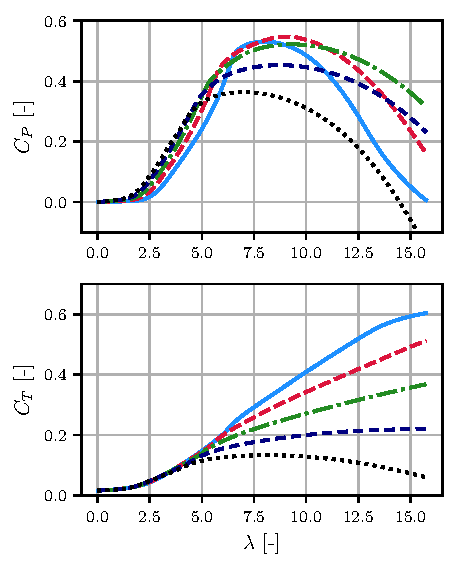
\includegraphics{validation/cp_ct.pdf}
	\caption{$\Phi =$ \legendFive{$-5$}{$-2.5$}{$0.0$}{$2.5$}{$5$.}
		$C_P$ and $C_T$ as functions of tip-speed ratio and pitch angle for the NREL 5MW turbine.}
	\label{fig:cp_+_ct}
\end{figure}
As a first step, the implementation of the BEM environment is validated. \autoref{fig:cp_+_ct} shows $C_P$ and $C_T$ computed as functions of the tip-speed ratio $\lambda$ and the collective pitch angle $\Phi$. The results appear reasonable compared to results given in \cite{hansen_aerodynamics_2008}, where a smaller turbine is used. For the NREL5 MW or any of the newer reference turbines data is not available. Furthermore, values obtained through interpolation of the precomputed table were compared to calculated values for $100$ tip-speed ratios. The difference was found to be of $\mathcal{O}\left(10^{-5}\right)$ or smaller, while the interpolation is $170$ times faster. \autoref{fig:cp_+_ct} shows that the power coefficient has a maximum between $\lambda=6$ and $\lambda=10.0$, depending on the pitch-angle. For $\Phi=0$, the maximum $C_P$ of $0.522$ occurs at $\lambda=9.23$. However, the thrust coefficient grows with tip-speed ratio for most pitch angles. The thrust influences the wake deficit and lifetime of wind turbines, therefore a reduction in $\lambda$ below the value maximizing $C_P$ can be advisable.\newpage
\begin{figure}[ht]
	\centering
	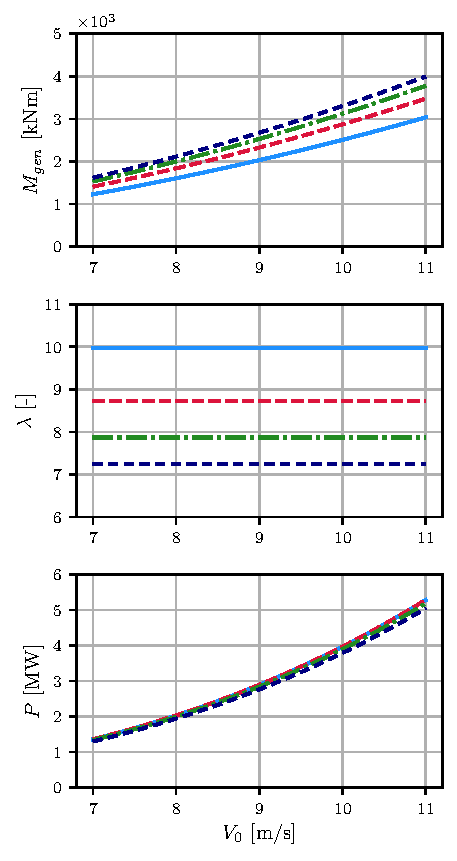
\includegraphics{validation/greedy.pdf}
	\caption{$\kappa =$ \legendFour{$1.0$}{$1.5$}{$2.0$}{$2.5 \, [\SI{1e6}{kgm^2}]$.}Controller curve of greedy controller for different values of the proportionality constant $\kappa$}
	\label{fig:controller_curve}
\end{figure}
To validate the greedy controller, the controller curve is computed in the BEM environment. It is shown in \autoref{fig:controller_curve}, for a range of values of $\kappa$. The choice of $\kappa$ has little influence on the power in comparison to the wind velocity $V_0$. However, the tip-speed ratio is greatly influenced by the choice of $\kappa$. As discussed above, tip-speed ratio influences $C_T$ and $C_P$. Thus a higher $\kappa$ can reduce the thrust exerted on the turbine, with only a small reduction in power. Comparing the controller curve to the curve given in \cite{jonkman_definition_2009}, a good agreement in $P$ and $M_{gen}$ is found for $\kappa=\SI{2.5e6}{kgm^2}$. However, since the lifetime of the turbine is not of concern, thus $\kappa$ maximizing $C_P$,  $\kappa = \SI{1.268e6}{kgm^2}$, is chosen. \\
\begin{figure}[h]
	\centering
	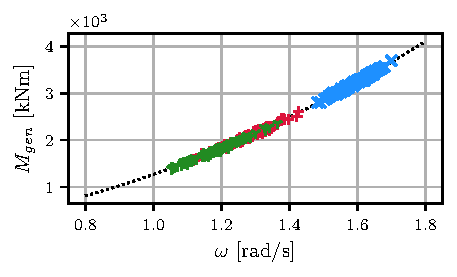
\includegraphics{validation/control.pdf}
	\caption{{\color{black} \rule[3pt]{1pt}{1pt} \rule[3pt]{1pt}{1pt} \rule[3pt]{1pt}{1pt} \rule[3pt]{1pt}{1pt} \rule[3pt]{1pt}{1pt} \rule[3pt]{1pt}{1pt}} $ \kappa \omega^2$
		{\color[HTML]{1E90FF} $\times$} Turbine 0
		{\color[HTML]{DC143C} $+$} Turbine 1
		{\color[HTML]{228B22} Y}
		Generator torque over angular velocity of three turbines controlled by greedy controller. Sampled every 200th timestep.}
	\label{fig:m_omega_greedy}
\end{figure}
The LBM-ALM with a constant angular velocity of the rotor has been validated by Asmuth et al. in \cite{asmuth_actuator_2019}. Therefore only the combination of the greedy controller with the LBM-ALM will be validated here. \autoref{fig:m_omega_greedy} shows $M_{gen}$ over $\omega$ for three turbines in a setup as described in \autoref{ssec:LBM_ALM_env}. The data gathered from the turbines agrees well with the expected value given by $\kappa \omega^2$. Deviations from the line are due to the turbulent inflow and the inertia of the turbine, but the figure shows, that the turbine can follow the changing conditions closely. Furthermore, the influence of the wake loss can be seen. While the first turbine operates near the values expected at rated wind speed, the second turbine has lower angular velocity and torque and thus generates less power. The third turbine has even lower values, although the difference between the second and third turbine is not as big as between the first and the second. \\
Thus the environments and the greedy controller exhibit the expected behaviour and the coupling of them is working as well. \newpage

	% !TEX root = ../../Diploma.tex
\section{Parameter Study}
\begin{figure}[ht]
	\centering
	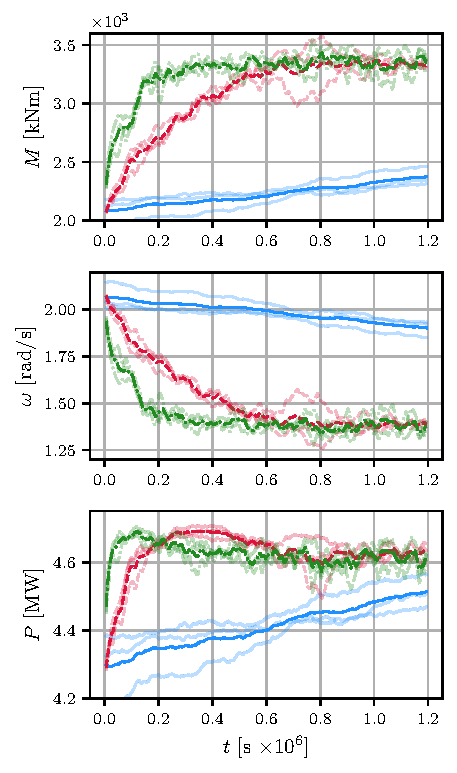
\includegraphics{parameter_study/variance.pdf}
	\caption{$\sigma_A=$ \legendThree{$0.01$}{$0.05$}{$0.1$.}Sensitivity of training to $\sigma_A$. Thin lines are individual trainings, thick lines are the average of all trainings.}
	\label{fig:var}
\end{figure}
To gain insight into the behaviour of the RL-agent and the influence of some of the parameters, a parameter study is conducted using the BEM environment. To reduce the effect of the random initialization of the networks, for each tested value of a parameter, three independent agents are trained. The evolution of generator torque, angular velocity and power throughout training for a fixed number of time steps is compared, since these values are used as action, state and reward, respectively. \\
First the influence of the variance of the action, $\sigma_A$ is studied. The results of the training for agents with variance of $0.01$, $0.05$ and $0.1$ are shown in \autoref{fig:var}. The comparison of the three values shows a clear trend. A higher variance leads to a faster increase in power. 
This can be expected, since a larger variance in the action leads to trying a wider range of actions. Therefore finding a coarse estimate of a beneficial behaviour is more likely. Furthermore, it is visible, that the two agents with a higher variance reach similar behaviour. This increases the confidence, that this behaviour represents a local optimum. However, they both reach a maximum of generated power in the first half of the training, but are not able to sustain that value throughout the rest of the training. Comparing the different agents with the same set of parameters show that stochastic variation is present in training of the agents.  After around two thirds of training time, one of agents with medium variance shows a significant drop in power, while another performs significantly better than average. However, towards the end of the training, the agents with medium variance perform more similar, more stable and slightly better than the agent with a higher variance. It can therefore be assumed that the choice of variance has to be a balance between a fast increase in the beginning and unstable behaviour in the end. It can be expected that the training of the agent controlling three turbines in the LBM-ALM environment will take significantly more time steps and the computational cost of a single time step is also much higher. Therefore, a faster increase is favoured and the variance is chosen to be $\sigma_A = 0.1$. \\
\begin{figure}[ht]
	\centering
	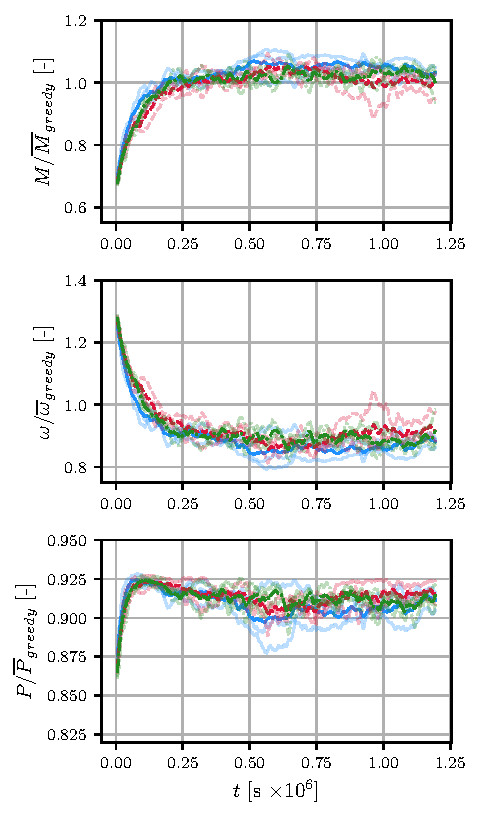
\includegraphics{parameter_study/policy_l2_reg.pdf}
	\caption{$\varepsilon_{p,l_2}=$ \legendThree{$0.0$}{$0.1$}{$0.2$.}Sensitivity of training to $\varepsilon_{p,l_2}$. Thin lines are individual trainings, thick lines are the average of all trainings.}
	\label{fig:p_l2}
\end{figure}
Next, the influence of an $l_2$-regularization of the policy network is examined. The results of the trainings without regularization and with regularization coefficients of $0.1$ and $0.2$ are shown in \autoref{fig:p_l2}. The sensitivity is significantly smaller to this parameter than to an increase in $\sigma_A$. While almost no difference is visible in the beginning for trainings with regularization, no regularization allows for a faster increase in power. However, on average, these agents drop the most afterwards. The agents also differ the most in power towards the end of the training. Remarkably, this is not the case for the generator torque, which differs most for $\varepsilon = 0.1$. A look back at \autoref{fig:cp_+_ct} shows, that near the optimum, $C_P$ is not very sensitive to changes in tip-speed ratio, which explains this discrepancy in action and reward. The optimal tip-speed ratio corresponds to an angular velocity of $\omega=\SI{1.58}{m/s}$. \autoref{fig:p_l2} shows that most of the agents operate at angular velocities below the optimum. The aforementioned agent sets a lower generator torque, therefore the angular velocity increases and is actually closer to the optimum. The difference in the case without regularization is caused by an increased torque, which has a bigger effect on $C_P$. In the last third of the training, the agents with $\varepsilon_{p,l_2}=0.1$ consistently perform best. Therefore this value is chosen. \\
\begin{figure}[h]%
	\centering
	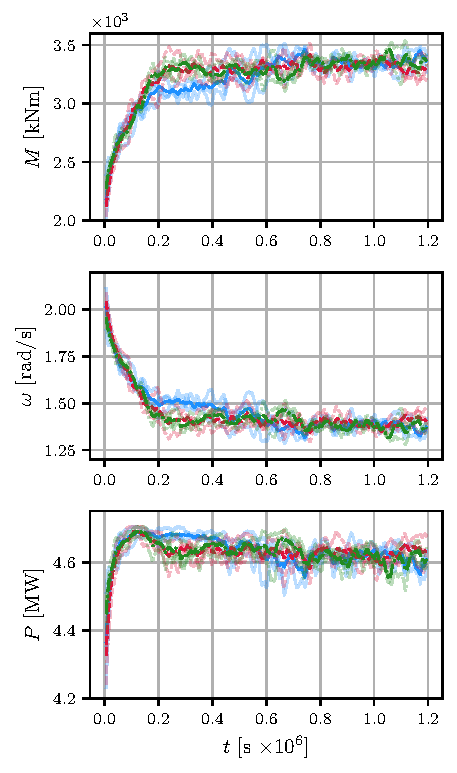
\includegraphics{parameter_study/value_function_l2_reg.pdf}
	\caption{$\varepsilon_{v,l_2}=$ \legendThree{$0.0$}{$0.1$}{$0.2$.}Sensitivity of training to $\varepsilon_{v,l_2}$. Thin lines are individual trainings, thick lines are the average of all trainings.}
	\label{fig:v_l2}
\end{figure}
Finally, the regularization of the value network is tested as well. The same coefficients as for the regularization of the policy network are tested. The sensitivity to a change in this parameter is similar to that of the policy regularization, as shown in \autoref{fig:p_l2}. A noticeable difference between the trainings is a delayed drop for trainings without regularization. However, this is only a delay. Later on the reductions in power are of similar magnitude as for the other cases, while the differences in generator torque are even larger than for the other agents. The second half of the training shows no clear trend for the best performance. The differences are small and the none of the averaged values is consistently better than the other. Since none of the tested values offers a clear advantage, the same value as for the regularization of the policy network is chosen.\\
The parameter study revealed a high sensitivity to a change in variance of the action and showed that an $l_2$-regularization benefits stability of the trained network while too much influence of the regularization might inhibit the optimization. In general, all of the studied trainings showed that the initial value of the generator torque is significantly lower than the optimal value. This is done by design, since a initial value that is too high leads to slowing down the turbine and a breakdown of $M_{aero}$, which ultimately makes a restart of the turbine necessary. Furthermore, almost all cases showed that $P$ reached a maximum value and then decreased. This was caused by a generator torque that is consistently set higher than what would be expected from a comparison with the controller curve of the greedy controller in \autoref{fig:controller_curve}. It can also already be noted that a lot of simulated time is necessary for the training of the agent. It can be expected that the necessary time will be at least similar, but probably more for the training of an agent controlling three turbines. \newpage

	\section{Optimizing Parameters of a Dynamic Behvaviour}
	\section{Learning a New Behaviour}
	\chapter{Conclusion}
	% !TEX root = ../Diploma.tex
In this work reinforcement learning was applied to control of a wind farm simulation utilizing the actuator line method and LES-LBM in order to increase the total generated power of the farm. Two approaches were tested. First, parameters of an already existing dynamic control strategy were improved. This was very successful, with an increase in total generated power by up to $18.2$ percent. Additionally, further insight into the physical phenomena of the dynamic control was gained. Second, the agent controlled the turbine directly. This approach was not able to improve total generated power and possible reasons for this were identified, among them the separation in time and space of the turbines. A possible solution of this problem by using multiple agents and environments was proposed. \\
In a first step, the theoretical basis for RL, ANNs, turbine modelling and control as well as LBM was laid. Also a more complete deduction for a second order refinement scheme for the cumulant LBM was given, which was not available in the literature. Furthermore a literature review of advanced dynamic induction control for wind farms and of active flow control via reinforcement learning was conducted. It was found, that the coupling of AFC and RL have only been conducted for laminar, two-dimensional problems. \\
In the second part, the framework developed for this work as well as details of the implementation and design choices were explained. Furthermore, the setup of the simulations was explained. The wind park features three turbines with a distance of five rotor diameters and turbulent inflow with a turbulence intensity of five percent. The different agents that were trained were also explained. Two agents were trained to improve the helix control strategy, which was taken from literature. One of the agents had a network of three layers with a width of 400 nodes, the other agents network consists of three layers with a width of ten nodes. Three agents were trained to learn a new control strategy by directly controlling the generator torque of the turbines. The training different in the length of the episodes, the first agent was trained with episodes of 1500 actions, the second and the third agent with episodes containing 500 actions. The return for the first and the second agent was discounted with a discount rate of $\gamma=0.99$, while the return for the third agent was discounted with a discount rate of $\gamma=0.95$. \\
Finally the results were discussed. First the implementation of the different parts of the simulations were validated. Then preliminary studies with a simple aerodynamic model of a single turbine were conducted. They showed that the training of an agent requires $\mathcal{O}(10^6\si{s})$ of simulated time. The results from the optimization of the parameters of the helix control strategy were discussed. The two agents resulted in similar behaviour with one difference. The agent with the smaller network set a negative amplitude, resulting in a phase shift of $\SI{180}{\degree}$ of the wake helix of the first turbine. With this shift an increase of $\SI{18.2}{}$ percent in total generated power was found, while the other agent, which did not feature the phase shift, resulted in an increase of $\SI{6.75}{}$ percent. It was found that this difference in total generated power was caused by a phase shift of the helix caused by the first turbine and the helix caused by the second turbine. In the first case, the helices were aligned, resulting in an increase of the radius of the helix. In the second case, the helices are shifted by $\SI{180}{\degree}$, which results in a destruction of the helix after the second turbine, decreasing power production at the second and the third turbine. Based on this finding it was proposed to shift the helix of the second turbine to align with the first turbine, which found an increase to that of the park controlled by agent with the small network. This provided further insight into the physical phenomena governing the helix approach, which had only been tested for a two-turbine park, of which only the first turbine was controlled with the helix approach. The findings in this work show how an application to a larger park can be offer significant increases in generated power.  \\
Lastly, the results of the training of the three agents directly controlling the generator torque of the turbines were evaluated. None of the agents were able to develop a strategy that performed better than a greedy-controlled park. Still, the analysis of the flow in a park controlled by one of the agents showed, that a slower reacting greedy controller might be able to reduce fluctuations in generated power. Three possible reasons were found why the agents could not find a good strategy in the current setup. All three agents developed a static strategy and did not react to the state of the environment any more. This was attributed to an inadequate transformation of the actions of the agent to the control quantities of the turbine. Three solutions were proposed. First, the a-priori values used for the transformation could be improved by using estimates based on greedy control. Second, an additional layer of linear nodes could be used in the network. Third, the agent could be trained to behave like a greedy controller by supervised learning. The second and third problem identified are related to the reward. On the one hand, the reward, which was defined to be the sum of the generated power of the three turbines, favours improving the first turbine, since this turbine produces the most power. Second, the control of the first turbine influences the second and third turbine but only after a long period of time. During this period of time, the control has no influence on the current state of the environment. If the influence on the downstream turbines is captured by the reward, it also includes many other time steps. If it is not captured, the optimization goal reduces to a greedy strategy. To tackle both of these problems it was proposed to change the setup to the use of a separate environment and agent for each turbine as well as modifying the the reward to include only time steps which can be relevant. \\
Three main conclusions regarding the application of RL to AFC can be drawn from this work. First, reinforcement learning coupled to active flow control requires a lot of simulated time, to apply it to three-dimensional, fully turbulent flows therefore is computationally very expensive. The cumulant LBM with the extension of second order refinement is a method well-suited for this task. Additionally, the hardware requirements of RL as well as LBM are similar, since both can be greatly accelerated by the use of GPUs. Second, applying RL to realistic problems requires many design choices from the great number of parameters in the learning algorithm to details in the implementation regarding non-dimensionalization. Since this was the first application of RL to such a realistic problem, no literature was available to rely on. Third, this methodology has the potential of discovering new control strategies or improving already existing strategies as well as hinting researchers at physical phenomena, which where not previously observed. \\
The results regarding the helix approach showed, that it has great potential to increase the power production of small wind parks but the newly gained understanding of the physics of this approach suggest that it can easily be extended to larger parks, if the phase shift of the helices is accounted for. To further prove the feasibility of this approach for control of real-world wind parks, simulations including a sheared boundary layer will have to be conducted, as the shear greatly influences the movement of the wake. Additionally a thorough study of the loads will be necessary, as they have only been assessed through thrust and aerodynamic moment until this point. \\
Future works on applying RL to wind farm control will have to solve the problems discussed above. Especially the problem of time shifted actions will have to be addressed to turn RL into a more useful tool for a broader range of problems. A possible solution to this was already suggested in this chapter. It might also be necessary to gain further understanding of RL in turbulent flows by studying simpler problems, such as a single turbine. The analysis of the control strategy developed by the RL-agent is further hindered by the black-box character of the neural network. To this end it might be feasible to use different approximation functions for the policy. The reduction of the state-space by applying a convolutional neural network or other order-reducing methods could also be a feasible addition to the approach taken in this work. Further there exist other methods of machine learning for non-linear control, such as Koopman operator theory, the application of these to wind-farm control can also be explored.
% 	\setlength{\abovedisplayskip}{16pt}		% größerer Abstand vor Equations
% 	\setlength{\belowdisplayskip}{16pt}		% größerer Abstand nach Equations
	\clearpage
	\renewcommand{\bibname}{Bibliography}
	\printbibliography
	\cleardoublepage
	\appendix
	\chapter{The Cumulant Lattice Boltzmann Method}
\section{Derivation of cumulants}
To provide a more detailed explanation of the cumulant lattice boltzmann method, a more thorough derivation is given here. First, the discrete distribution is written as in a continuous form as shown in \eqref{eq:contin}. This is transformed to frequency space, to ensure Galilean Invariance as shown in \eqref{eq:cum_laplace}. This distribution is then used in the cumulant generating function, displayed in \eqref{eq:cum}. However, from that form, the cumulants are not directly computable. Comparing the cumulant generating function to the moment generating function in \eqref{eq:moments} shows their similarity. Computing the cumulants of a arbitrary function shows how they can be expressed in terms of moments, two examples for second order cumulants are given in \eqref{eq:c_200} and \eqref{eq:c_110}. Cumulants can also be computed from central moments, which is requires less computations \cite{geier_cumulant_2015}. Cumulants of zeroth and first order stay constant throughout the collision. The cumulants upwards from order two can now be relaxed indivdually like \eqref{eq:relax}, therefore each has its own relaxation frequency. The first frequency $\omega_1$ governs the shear viscosity and $\omega_2$ the bulk viscosity of the fluid by the same relation as \eqref{eq:nu}. The rest of the frequencies can be chosen freely and are usually set to one, resulting fully relaxing the cumulants, however a parametrized version of the collision operation exists, that changes some of the higher order relaxation frequencies, leading to fourth order accurate diffusion in a fully resolved simulation \cite{geier_parametrization_2017}. In underresolved simulations the parameter introduced in the parametrization can be used to influence the diffusivity and therefore acting as an implicit subgrid scale model, however so far only empirical evidence exists for this.\cite{geier_cumulant_2015} 
\begin{align}
f(\xi, \upsilon, \zeta) &= \sum_{i,j,k} f_{i,j,k} \delta(ic_s - \xi) \delta(jc_s - \upsilon) \delta(kc_s - \zeta) \label{eq:contin}\\
F(\vec{\Xi}) &= \int_{-\infty}^{\infty}f(\xi, \upsilon, \zeta)e^{-\vec{\Xi} \cdot \vec{\xi}} \mathrm{d}\vec{\xi} \label{eq:cum_laplace} \\
M_{\alpha, \beta, \gamma} &= c_s^{-(\alpha+\beta+\gamma)} \left. \frac{\partial^\alpha \partial^\beta \partial^\gamma}{\partial \Xi^\alpha \partial \Upsilon^\beta \partial Z^\gamma} F(\Xi, \Upsilon, Z) \right|_{\Xi=\Upsilon=Z=0} = \sum_{i,j,k} i^\alpha j^\beta k^\gamma f_{i,j,k} \label{eq:moments}\\
C_{\alpha,\beta,\gamma} &= c_s^{-(\alpha+\beta+\gamma)} \left. \frac{\partial^\alpha \partial^\beta \partial^\gamma}{\partial \Xi^\alpha \partial \Upsilon^\beta \partial Z^\gamma} \ln F(\Xi, \Upsilon, Z)\right|_{\Xi=\Upsilon=Z=0} \label{eq:cum} \\
C_{200} &= \frac{M_{200}}{M_{000}} - \frac{M_{100}^2}{M_{000}^2} \label{eq:c_200}\\
C_{110} &= \frac{M_{110}}{M_{000}} - \frac{M_{100} M_{010}}{M_{000}^2} \label{eq:c_110} \\
C_{\alpha, \beta, \gamma}* &= \left(1-\omega_{\alpha,\beta,\gamma}\right) C_{\alpha, \beta, \gamma} \label{eq:relax}
\end{align}
In addition, the density, velocity and the terms of velocity gradient tensor can be identified with cumulants as shown in \eqref{eq:drho} - \eqref{eq:derivative2}. Note, that in this derivation the well-conditioned cumulant is used as described in the appendix of \cite{geier_cumulant_2015} and therefore the zeroth order cumulant is not the density but its deviation from unit density $\delta \rho$. Also the additional moments $k_{xy}$ and $k_{xx-yy}$ are introduced for use in the chapter on refinement.
\begin{align}
\delta \rho &= M_{000} = C_{000} \label{eq:drho}\\
u &= \frac{M_{100}}{M_{000}} =  C_{100}\\
D_x v + D_y u &= -3 \omega_1 C_{110} = k_{xy} \label{eq:derivate1}\\
D_x u &= - \frac{\omega_1}{2 \rho}\left(2 C_{200} - C_{020} - C_{002} \right) - \frac{\omega_2}{2 \rho} \left(C_{200} + C_{020} + C_{002} - \delta \rho \right) \\
D_x u - D_y v &= - \frac{3\omega_1}{2} \left(C_{200} - C_{020}\right) = k_{xx-yy}\label{eq:derivative2}
\end{align}
\section{Refinement}
As was stated before, LBM is usually used on a uniform grid. However, often a variation in grid spacing is desirable, as coarser grids need less memory and have a coarser timestep, whereas a finer grid is able to resolve finer turbulent structures. To balance these two interests, the domain can be partitioned into blocks with different levels of refinement, as areas of high turbulence, which need high resolution, usually occur only in known parts of the domain. The question is now how to treat the borders of the blocks. In \cite{schonherr_towards_2015} the compact interpolation scheme is proposed that is second order accurate, therefore it is consistent with the order of accuracy of the LBM in general. However, the derivation given was found to be neither exhaustive, nor fully correct, as there seem to be misprints, making it difficult to follow. Therefore a more detailed derivation is given here, that is based on \cite{schonherr_towards_2015} as well as \cite{kutscher_multiscale_2019}, which gave a version for an incompressible form of LBM, but suffers from similar issues. In each coarse timestep, a layer of coarse nodes is interpolated from fine nodes and two layers of fine nodes are interpolated from coarse nodes. The node being interpolated is called the receiver node while the nodes from which is interpolated is referred to as the donor node. Each receiver node has eight donor nodes. A local coordinate system in the center of cube is defined, with the donor nodes laying in the corners at $x={-0.5, 0.5}$, $y={-0.5,0.5}$ and $z={-0.5,0.5}$. \\First, a interpolation function for the density, $\delta \hat{\rho}$ and the velocities $\hat{u}$, $\hat{v}$ and $\hat{w}$ is defined. Note that the density only requires to be first order accurate.
\begin{align}
	 \delta \hat{\rho} &= d_0 + d_x x + d_y y + d_z z + d_{xy}xy + d_{xz}xz + d_{yz}yz + d_{xyz}xyz \\
	\hat{u} &= a_0 + a_x x + a_y y + a_z z + a_{xx} x^2 + a_{xy} xy + a_{xz} xz + a_{yy} y^2 + a_{yz} yz + a_{zz} z^2 + a_{xyz}xyz \\
	\hat{v} &= b_0 + b_x x + b_y y + b_z z + b_{xx} x^2 + b_{xy} xy + b_{xz} xz + b_{yy} y^2 + b_{yz} yz + b_{zz} z^2 + b_{xyz}xyz \\
	\hat{w} &= c_0 + c_x x + c_y y + c_z z + c_{xx} x^2 + c_{xy} xy + c_{xz} xz + c_{yy} y^2 + c_{yz} yz + c_{zz} z^2 + c_{xyz}xyz
\end{align}
To evualate the interpolation functions, constraints have to be defined. The velocity and density in the donor node place 32 constraints, since there are eight of each, thus nine more are required for the 41 degrees of freedom. The second derivative of velocities in the center of the local coordinate system are chosen. They can be computed by taking the first order central difference of the terms of the velocity gradient tensor. However, the terms in the main diagonal of the velocity gradient tensor are lengthy and include $\omega_2$. This is somewhat undesirable and it was shown in \eqref{eq:derivate1} that differences of the terms can be expressed more directly. Therefore the remaining nine constraints are chosen like shown in \eqref{eq:const1} - \eqref{eq:const2}, the missing five constraints by the off diagonal can easily be extrapolated.
\begin{align}
	\frac{\partial^2}{\partial x^2} \hat{v}+\frac{\partial^2}{\partial y \partial x} \hat{u} &= D_{xx} v + D_{xy} u \label{eq:const1} \\
	2\frac{\partial^2}{\partial x^2} \hat{u} - \frac{\partial^2}{\partial x \partial y} \hat{v} - \frac{\partial^2}{\partial x \partial z} \hat{w} &= 2 D_{xx}u- D_{xy}v - D_{xz}w \\
	2\frac{\partial^2}{\partial y^2} \hat{v} - \frac{\partial^2}{\partial x \partial y} \hat{u} - \frac{\partial^2}{\partial y \partial z} \hat{w} &= 2 D_{yy}v- D_{xy}u - D_{yz}w \\
	2\frac{\partial^2}{\partial z^2} \hat{w} - \frac{\partial^2}{\partial y \partial z} \hat{v} - \frac{\partial^2}{\partial x \partial z} \hat{u} &= 2 D_{zz}w- D_{yz}v - D_{xz}u \label{eq:const2}
\end{align}
Thus a system of linear equations is established that can be solved for the coefficients of the interpolation functions. They are listed below, in order to reduce the number length of equations only unique descriptions are given, the other coefficients can easily extrapolated. 
\begin{align}
	a_0 &= \frac{1}{32} \sum_{x,y,z}  -4 D_{xx}u-2 D_{xy}v -4D_{yy}u- 2 D_{xz}w + -4 D_{zz}u + 4 u_{xyz} + 4xyv_{xyz} + 4 xzw_{xyz} \\
	&= \frac{1}{32} \sum_{x,y,z}  -x\left(k_{xx-yy} + k_{xx-zz}\right) - 2yk_{xy} -2zk_{xz} + 4 u_{xyz} + 4xyv_{xyz} + 4 xzw_{xyz} \\
	a_x &= \frac{1}{2} \sum_{x,y,z} x u_{xyz} \\
	a_{xx} &= \frac{1}{8} \sum_{x,y,z}x\left(k_{xx-yy}+k_{xx-zz}\right) + 4xyv_{xyz}+ 4 xzw_{xyz} \\
	a_{yy} &= \frac{1}{8} \sum_{x,y,z}y k_{xy} - 4 xy v_{xyz} \\
	a_{xy} &= 2 \sum_{x,y,z} xyu_{xyz} \\
	a_{xyz} &= 8 \sum_{x,y,z} xyzu_{xyz} \\
	d_0 &= \frac{1}{8} \sum_{x,y,z} \delta \rho_{xyz} 
\end{align}
Thus the velocities are computed to second order. To arrive at equations for the second order cumulants, \eqref{eq:derivate1} - \eqref{eq:derivative2} are solved for cumulants. A term including the divergence of the velocity is neglected, since LBM is valid in a weakly compressible range and the term is thus much smaller.To compute the cumulants, the derivatves of $\hat{u}$, $\hat{v}$ and $\hat{w}$ are used and the constant terms in the derivatives are replaced with averaged values of second order moments. Also $\omega_1$ has to be scaled with a factor $\sigma$ to account for the change in refinement, it is $2$ when scaling from fine to coarse and $1/2$ when scaling from coarse to fine. 
\begin{align}
	A_{011} &= \frac{\partial \hat{v}}{\partial z} + \frac{\partial \hat{w}}{\partial y} - b_z - c_y \\
	&= b_{xz} x + b_{yz} y + 2 b_{zz} z + b_{xyz} xy + c_{xy} x + 2 c_{yy} y + c_{yz} z + c_{xyz} xz \\
	A_{101} &= \frac{\partial \hat{u}}{\partial z} + \frac{\partial \hat{w}}{\partial x} - a_z - c_x \\
	&= a_{xz} x + a_{yz} y + 2 a_{zz} z + a_{xyz} xy + 2 c_{xx} x + c_{xy} y + c_{xz} z + c_{xyz} yz \\
	A_{110} &= \frac{\partial \hat{u}}{\partial y} + \frac{\partial \hat{v}}{\partial x} - a_y - b_x \\
	&= a_{xy} x + 2 a_{yy} y + a_{yz} z + a_{xyz} xz + 2 b_{xx} x + b_{xy} y + b_{xz} z + b_{xyz} yz \\
	B &= \frac{\partial \hat{u}}{\partial x} - \frac{\partial \hat{v}}{\partial y} - a_x + b_y \\
	&= 2 a_{xx} x + a_{xy} y + a_{xz} z + a_{xyz} yz - b_{xy} x - 2 b_{yy} y - b_{yz} z - b_{xyz} xz \\
	C &= \frac{\partial \hat{u}}{\partial x} - \frac{\partial \hat{w}}{\partial z} - a_x + c_z \\
	&= 2 a_{xx} x + a_{xy} y + a_{xz} z + a_{xyz} yz - c_{xz} x - c_{yz} y - 2 c_{zz} y - c_{xyz} xy\\
	C_{011} &= - \frac{\sigma \rho}{3 \omega_d} \left( \overline{k_{yz}} + A_{011} \right)\\
	C_{101} &= - \frac{\sigma \rho}{3 \omega_d} \left( \overline{k_{xz}} + A_{101} \right) \\
	C_{110} &= - \frac{\sigma \rho}{3 \omega_d} \left( \overline{k_{xy}} + A_{110} \right) \\
	C_{200} &= \frac{\delta \rho}{9} - \frac{2 \sigma \rho}{9 \omega_d} \left( \overline{k_{xx-yy}} + B + \overline{k_{xx-zz}} + C \right) \\
	C_{020} &= \frac{\delta \rho}{9} - \frac{2 \sigma \rho}{9 \omega_d} \left( -2 \left(\overline{k_{xx-yy}} + B\right) + \overline{k_{xx-zz}} + C \right) \\
	C_{002} &= \frac{\delta \rho}{9} - \frac{2 \sigma \rho}{9 \omega_d} \left( \overline{k_{xx-yy}} + B - 2 \left( \overline{k_{xx-zz}} + C \right) \right)		
\end{align}
Now the cumulants can be transformed back to distributions, with the central moments up to order two and cumulants of order higher than two set to zero. 
	\cleardoublepage
\chapter*{Selbstständigkeitserklärung}
\thispagestyle{empty}
Hiermit erkläre ich, dass ich die von mir am heutigen Tag der Professur für Strömungsmechanik eingereichte 
%Diplomarbeit
Interdisziplinäre Projektarbeit 
%(den) Großen Beleg (eingereichten)
zum Thema 
\begin{center}
\textit{Validierung eines Wandmodels für Large Eddy Simulationen auf der Basis der Lattice-Boltzmann Methode}
\end{center}
vollkommen selbstständig verfasst und keine anderen als die angegebenen Quellen und Hilfsmittel benutzt, sowie Zitate kenntlich gemacht habe.
\\[10mm]
Dresden, 06. Januar 2020 \\[1cm]
Henry Korb


\end{document}